\documentclass[1p]{elsarticle_modified}
%\bibliographystyle{elsarticle-num}

%\usepackage[colorlinks]{hyperref}
%\usepackage{abbrmath_seonhwa} %\Abb, \Ascr, \Acal ,\Abf, \Afrak
\usepackage{amsfonts}
\usepackage{amssymb}
\usepackage{amsmath}
\usepackage{amsthm}
\usepackage{scalefnt}
\usepackage{amsbsy}
\usepackage{kotex}
\usepackage{caption}
\usepackage{subfig}
\usepackage{color}
\usepackage{graphicx}
\usepackage{xcolor} %% white, black, red, green, blue, cyan, magenta, yellow
\usepackage{float}
\usepackage{setspace}
\usepackage{hyperref}

\usepackage{tikz}
\usetikzlibrary{arrows}

\usepackage{multirow}
\usepackage{array} % fixed length table
\usepackage{hhline}

%%%%%%%%%%%%%%%%%%%%%
\makeatletter
\renewcommand*\env@matrix[1][\arraystretch]{%
	\edef\arraystretch{#1}%
	\hskip -\arraycolsep
	\let\@ifnextchar\new@ifnextchar
	\array{*\c@MaxMatrixCols c}}
\makeatother %https://tex.stackexchange.com/questions/14071/how-can-i-increase-the-line-spacing-in-a-matrix
%%%%%%%%%%%%%%%

\usepackage[normalem]{ulem}

\newcommand{\msout}[1]{\ifmmode\text{\sout{\ensuremath{#1}}}\else\sout{#1}\fi}
%SOURCE: \msout is \stkout macro in https://tex.stackexchange.com/questions/20609/strikeout-in-math-mode

\newcommand{\cancel}[1]{
	\ifmmode
	{\color{red}\msout{#1}}
	\else
	{\color{red}\sout{#1}}
	\fi
}

\newcommand{\add}[1]{
	{\color{blue}\uwave{#1}}
}

\newcommand{\replace}[2]{
	\ifmmode
	{\color{red}\msout{#1}}{\color{blue}\uwave{#2}}
	\else
	{\color{red}\sout{#1}}{\color{blue}\uwave{#2}}
	\fi
}

\newcommand{\Sol}{\mathcal{S}} %segment
\newcommand{\D}{D} %diagram
\newcommand{\A}{\mathcal{A}} %arc


%%%%%%%%%%%%%%%%%%%%%%%%%%%%%5 test

\def\sl{\operatorname{\textup{SL}}(2,\Cbb)}
\def\psl{\operatorname{\textup{PSL}}(2,\Cbb)}
\def\quan{\mkern 1mu \triangleright \mkern 1mu}

\theoremstyle{definition}
\newtheorem{thm}{Theorem}[section]
\newtheorem{prop}[thm]{Proposition}
\newtheorem{lem}[thm]{Lemma}
\newtheorem{ques}[thm]{Question}
\newtheorem{cor}[thm]{Corollary}
\newtheorem{defn}[thm]{Definition}
\newtheorem{exam}[thm]{Example}
\newtheorem{rmk}[thm]{Remark}
\newtheorem{alg}[thm]{Algorithm}

\newcommand{\I}{\sqrt{-1}}
\begin{document}

%\begin{frontmatter}
%
%\title{Boundary parabolic representations of knots up to 8 crossings}
%
%%% Group authors per affiliation:
%\author{Yunhi Cho} 
%\address{Department of Mathematics, University of Seoul, Seoul, Korea}
%\ead{yhcho@uos.ac.kr}
%
%
%\author{Seonhwa Kim} %\fnref{s_kim}}
%\address{Center for Geometry and Physics, Institute for Basic Science, Pohang, 37673, Korea}
%\ead{ryeona17@ibs.re.kr}
%
%\author{Hyuk Kim}
%\address{Department of Mathematical Sciences, Seoul National University, Seoul 08826, Korea}
%\ead{hyukkim@snu.ac.kr}
%
%\author{Seokbeom Yoon}
%\address{Department of Mathematical Sciences, Seoul National University, Seoul, 08826,  Korea}
%\ead{sbyoon15@snu.ac.kr}
%
%\begin{abstract}
%We find all boundary parabolic representation of knots up to 8 crossings.
%
%\end{abstract}
%\begin{keyword}
%    \MSC[2010] 57M25 
%\end{keyword}
%
%\end{frontmatter}

%\linenumbers
%\tableofcontents
%
\newcommand\colored[1]{\textcolor{white}{\rule[-0.35ex]{0.8em}{1.4ex}}\kern-0.8em\color{red} #1}%
%\newcommand\colored[1]{\textcolor{white}{ #1}\kern-2.17ex	\textcolor{white}{ #1}\kern-1.81ex	\textcolor{white}{ #1}\kern-2.15ex\color{red}#1	}

{\Large $\underline{12n_{0553}~(K12n_{0553})}$}

\setlength{\tabcolsep}{10pt}
\renewcommand{\arraystretch}{1.6}
\vspace{1cm}\begin{tabular}{m{100pt}>{\centering\arraybackslash}m{274pt}}
\multirow{5}{120pt}{
	\centering
	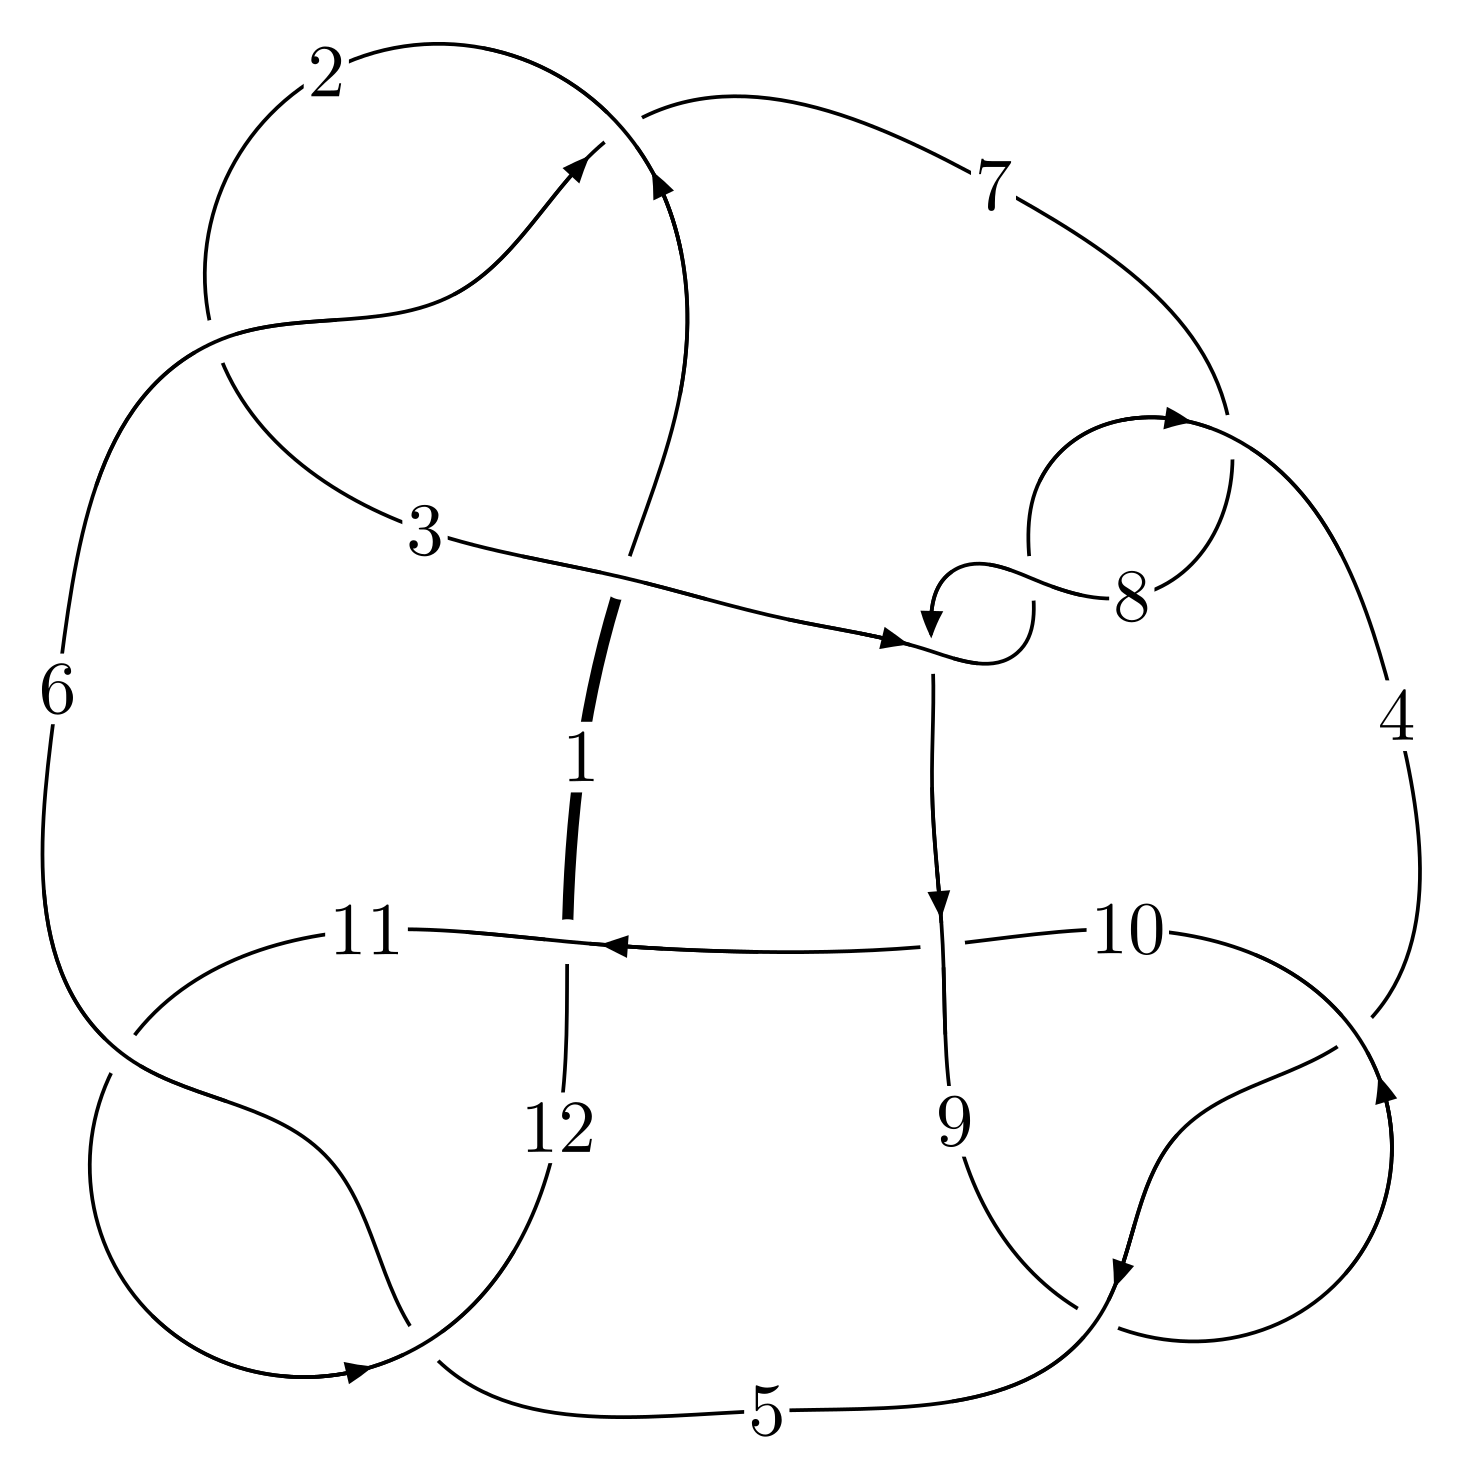
\includegraphics[width=112pt]{../../../GIT/diagram.site/Diagrams/png/2642_12n_0553.png}\\
\ \ \ A knot diagram\footnotemark}&
\allowdisplaybreaks
\textbf{Linearized knot diagam} \\
\cline{2-2}
 &
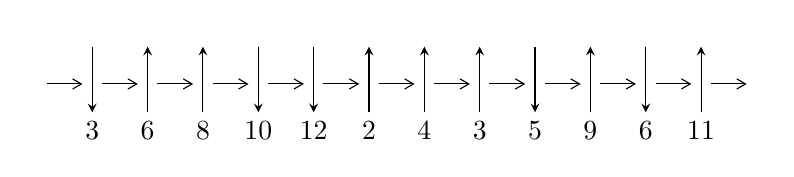
\begin{tikzpicture}[x=20pt, y=17pt]
	% nodes
	\node (C0) at (0, 0) {};
	\node (C1) at (1, 0) {};
	\node (C1U) at (1, +1) {};
	\node (C1D) at (1, -1) {3};

	\node (C2) at (2, 0) {};
	\node (C2U) at (2, +1) {};
	\node (C2D) at (2, -1) {6};

	\node (C3) at (3, 0) {};
	\node (C3U) at (3, +1) {};
	\node (C3D) at (3, -1) {8};

	\node (C4) at (4, 0) {};
	\node (C4U) at (4, +1) {};
	\node (C4D) at (4, -1) {10};

	\node (C5) at (5, 0) {};
	\node (C5U) at (5, +1) {};
	\node (C5D) at (5, -1) {12};

	\node (C6) at (6, 0) {};
	\node (C6U) at (6, +1) {};
	\node (C6D) at (6, -1) {2};

	\node (C7) at (7, 0) {};
	\node (C7U) at (7, +1) {};
	\node (C7D) at (7, -1) {4};

	\node (C8) at (8, 0) {};
	\node (C8U) at (8, +1) {};
	\node (C8D) at (8, -1) {3};

	\node (C9) at (9, 0) {};
	\node (C9U) at (9, +1) {};
	\node (C9D) at (9, -1) {5};

	\node (C10) at (10, 0) {};
	\node (C10U) at (10, +1) {};
	\node (C10D) at (10, -1) {9};

	\node (C11) at (11, 0) {};
	\node (C11U) at (11, +1) {};
	\node (C11D) at (11, -1) {6};

	\node (C12) at (12, 0) {};
	\node (C12U) at (12, +1) {};
	\node (C12D) at (12, -1) {11};
	\node (C13) at (13, 0) {};

	% arrows
	\draw[->,>={angle 60}]
	(C0) edge (C1) (C1) edge (C2) (C2) edge (C3) (C3) edge (C4) (C4) edge (C5) (C5) edge (C6) (C6) edge (C7) (C7) edge (C8) (C8) edge (C9) (C9) edge (C10) (C10) edge (C11) (C11) edge (C12) (C12) edge (C13) ;	\draw[->,>=stealth]
	(C1U) edge (C1D) (C2D) edge (C2U) (C3D) edge (C3U) (C4U) edge (C4D) (C5U) edge (C5D) (C6D) edge (C6U) (C7D) edge (C7U) (C8D) edge (C8U) (C9U) edge (C9D) (C10D) edge (C10U) (C11U) edge (C11D) (C12D) edge (C12U) ;
	\end{tikzpicture} \\
\hhline{~~} \\& 
\textbf{Solving Sequence} \\ \cline{2-2} 
 &
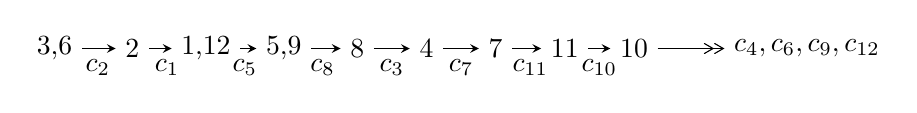
\begin{tikzpicture}[x=25pt, y=7pt]
	% node
	\node (A0) at (-1/8, 0) {3,6};
	\node (A1) at (1, 0) {2};
	\node (A2) at (33/16, 0) {1,12};
	\node (A3) at (51/16, 0) {5,9};
	\node (A4) at (17/4, 0) {8};
	\node (A5) at (21/4, 0) {4};
	\node (A6) at (25/4, 0) {7};
	\node (A7) at (29/4, 0) {11};
	\node (A8) at (33/4, 0) {10};
	\node (C1) at (1/2, -1) {$c_{2}$};
	\node (C2) at (3/2, -1) {$c_{1}$};
	\node (C3) at (21/8, -1) {$c_{5}$};
	\node (C4) at (15/4, -1) {$c_{8}$};
	\node (C5) at (19/4, -1) {$c_{3}$};
	\node (C6) at (23/4, -1) {$c_{7}$};
	\node (C7) at (27/4, -1) {$c_{11}$};
	\node (C8) at (31/4, -1) {$c_{10}$};
	\node (A9) at (43/4, 0) {$c_{4},c_{6},c_{9},c_{12}$};

	% edge
	\draw[->,>=stealth]	
	(A0) edge (A1) (A1) edge (A2) (A2) edge (A3) (A3) edge (A4) (A4) edge (A5) (A5) edge (A6) (A6) edge (A7) (A7) edge (A8) ;
	\draw[->>,>={angle 60}]	
	(A8) edge (A9);
\end{tikzpicture} \\ 

\end{tabular} \\

\footnotetext{
The image of knot diagram is generated by the software ``\textbf{Draw programme}" developed by Andrew Bartholomew(\url{http://www.layer8.co.uk/maths/draw/index.htm\#Running-draw}), where we modified some parts for our purpose(\url{https://github.com/CATsTAILs/LinksPainter}).
}\phantom \\ \newline 
\centering \textbf{Ideals for irreducible components\footnotemark of $X_{\text{par}}$} 
 
\begin{align*}
I^u_{1}&=\langle 
- u^6-4 u^4- u^3-3 u^2+2 d- u,\;u^7- u^6+4 u^5-3 u^4+2 u^3-4 u^2+4 c-3 u-4,\;b- u,\\
\phantom{I^u_{1}}&\phantom{= \langle  }- u^6-4 u^4-3 u^3-3 u^2+2 a-7 u-2,\;u^8+5 u^6+3 u^5+7 u^4+8 u^3+5 u^2+u+2\rangle \\
I^u_{2}&=\langle 
- u^4- u^2+d+u+1,\;- u^5- u^4- u^3- u^2+4 c+2 u,\;u^5- u^4+3 u^3-3 u^2+2 b+4 u-2,\\
\phantom{I^u_{2}}&\phantom{= \langle  }u^5- u^4+3 u^3- u^2+4 a+4 u,\;u^6- u^5+3 u^4-5 u^3+4 u^2-4 u+4\rangle \\
I^u_{3}&=\langle 
c u+d-1,\;c^2+3 u^2+c+2 u+9,\;b- u,\;a+1,\;u^3+u^2+3 u+1\rangle \\
I^u_{4}&=\langle 
- u^2+d,\;c-1,\;b- u,\;- u^3+a-2 u-1,\;u^4- u^3+3 u^2-2 u+1\rangle \\
I^u_{5}&=\langle 
- u^2+d,\;c-1,\;u^2+b,\;- u^3+2 u^2+a- u,\;u^4- u^3+u^2+1\rangle \\
I^u_{6}&=\langle 
- u^2+d,\;c-1,\;u^3+u^2+b+2 u+1,\;u^3+2 a+u-1,\;u^4+2 u^3+3 u^2+3 u+2\rangle \\
I^u_{7}&=\langle 
- u^3+u^2+d-2 u+1,\;- u^3+c-2 u,\;b- u,\;- u^3+a-2 u-1,\;u^4- u^3+3 u^2-2 u+1\rangle \\
I^u_{8}&=\langle 
- u^3+u^2+d-2 u+1,\;- u^3+c-2 u,\;- u^3+u^2+b-2 u+1,\;-2 u^3+2 u^2+a-5 u+3,\\
\phantom{I^u_{8}}&\phantom{= \langle  }u^4- u^3+3 u^2-2 u+1\rangle \\
I^u_{9}&=\langle 
- u^3+u^2+d-2 u+1,\;- u^3+c-2 u,\;u^3- u^2+b+3 u-1,\;a+1,\;u^4- u^3+3 u^2-2 u+1\rangle \\
I^u_{10}&=\langle 
u^3+d+1,\;u^3+2 c+u+1,\;u^3+u^2+b+2 u+1,\;u^3+2 a+u-1,\;u^4+2 u^3+3 u^2+3 u+2\rangle \\
\end{align*}\\
\begin{align*}
I^u_{11}&=\langle 
2 u^3-2 u^2+d+5 u-4,\;u^3+c+2 u+1,\;u^3- u^2+b+3 u-1,\;a+1,\;u^4- u^3+3 u^2-2 u+1\rangle \\
I^u_{12}&=\langle 
d- u+1,\;c-1,\;b,\;a- u,\;u^2+1\rangle \\
I^u_{13}&=\langle 
d+1,\;c,\;b+u,\;a-1,\;u^2+1\rangle \\
I^u_{14}&=\langle 
d+u+1,\;c-1,\;b+u,\;a-1,\;u^2+1\rangle \\
I^u_{15}&=\langle 
d a+a+u+1,\;c-1,\;b+u,\;u^2+1\rangle \\
\\
I^v_{1}&=\langle 
a,\;d-1,\;- a v+c- v-1,\;b+v,\;v^2+1\rangle \\
\end{align*}
\raggedright * 15 irreducible components of $\dim_{\mathbb{C}}=0$, with total 60 representations.\\
\raggedright * 1 irreducible components of $\dim_{\mathbb{C}}=1$ \\
\footnotetext{All coefficients of polynomials are rational numbers. But the coefficients are sometimes approximated in decimal forms when there is not enough margin.}
\newpage
\renewcommand{\arraystretch}{1}
\centering \section*{I. $I^u_{1}= \langle - u^6-4 u^4+\cdots+2 d- u,\;u^7- u^6+\cdots+4 c-4,\;b- u,\;- u^6-4 u^4+\cdots+2 a-2,\;u^8+5 u^6+\cdots+u+2 \rangle$}
\flushleft \textbf{(i) Arc colorings}\\
\begin{tabular}{m{7pt} m{180pt} m{7pt} m{180pt} }
\flushright $a_{3}=$&$\begin{pmatrix}1\\0\end{pmatrix}$ \\
\flushright $a_{6}=$&$\begin{pmatrix}0\\u\end{pmatrix}$ \\
\flushright $a_{2}=$&$\begin{pmatrix}1\\u^2\end{pmatrix}$ \\
\flushright $a_{1}=$&$\begin{pmatrix}u^2+1\\u^2\end{pmatrix}$ \\
\flushright $a_{12}=$&$\begin{pmatrix}-\frac{1}{4} u^7+\frac{1}{4} u^6+\cdots+\frac{3}{4} u+1\\\frac{1}{2} u^6+2 u^4+\frac{1}{2} u^3+\frac{3}{2} u^2+\frac{1}{2} u\end{pmatrix}$ \\
\flushright $a_{5}=$&$\begin{pmatrix}\frac{1}{4} u^7-\frac{1}{4} u^6+\cdots+2 u^2+\frac{1}{4} u\\-\frac{1}{4} u^7+\frac{1}{4} u^6+\cdots+\frac{1}{4} u+\frac{1}{2}\end{pmatrix}$ \\
\flushright $a_{9}=$&$\begin{pmatrix}\frac{1}{2} u^6+2 u^4+\cdots+\frac{7}{2} u+1\\u\end{pmatrix}$ \\
\flushright $a_{8}=$&$\begin{pmatrix}\frac{1}{2} u^6+2 u^4+\cdots+\frac{5}{2} u+1\\u\end{pmatrix}$ \\
\flushright $a_{4}=$&$\begin{pmatrix}-\frac{1}{2} u^7-2 u^5+\cdots- u+1\\- u^2\end{pmatrix}$ \\
\flushright $a_{7}=$&$\begin{pmatrix}u\\u^3+u\end{pmatrix}$ \\
\flushright $a_{11}=$&$\begin{pmatrix}-\frac{1}{4} u^7+\frac{1}{4} u^6+\cdots+\frac{3}{4} u+1\\-\frac{1}{4} u^7+\frac{1}{4} u^6+\cdots+\frac{1}{4} u+\frac{1}{2}\end{pmatrix}$ \\
\flushright $a_{10}=$&$\begin{pmatrix}\frac{1}{4} u^7+\frac{1}{4} u^6+\cdots+\frac{11}{4} u+1\\-\frac{1}{2} u^6- u^4+\cdots+\frac{1}{2} u^2+\frac{1}{2} u\end{pmatrix}$\\&\end{tabular}
\flushleft \textbf{(ii) Obstruction class $= -1$}\\~\\
\flushleft \textbf{(iii) Cusp Shapes $= - u^7- u^6-2 u^5-9 u^4-12 u^2-9 u$}\\~\\
\newpage\renewcommand{\arraystretch}{1}
\flushleft \textbf{(iv) u-Polynomials at the component}\newline \\
\begin{tabular}{m{50pt}|m{274pt}}
Crossings & \hspace{64pt}u-Polynomials at each crossing \\
\hline $$\begin{aligned}c_{1}\end{aligned}$$&$\begin{aligned}
&u^8+10 u^7+39 u^6+71 u^5+55 u^4+20 u^3+37 u^2+19 u+4
\end{aligned}$\\
\hline $$\begin{aligned}c_{2},c_{3},c_{6}\\c_{7},c_{8}\end{aligned}$$&$\begin{aligned}
&u^8+5 u^6+3 u^5+7 u^4+8 u^3+5 u^2+u+2
\end{aligned}$\\
\hline $$\begin{aligned}c_{4},c_{5},c_{9}\\c_{11}\end{aligned}$$&$\begin{aligned}
&u^8+u^6+3 u^5+3 u^4+5 u^2+u+2
\end{aligned}$\\
\hline $$\begin{aligned}c_{10},c_{12}\end{aligned}$$&$\begin{aligned}
&u^8-2 u^7+7 u^6-7 u^5+23 u^4-28 u^3+37 u^2-19 u+4
\end{aligned}$\\
\hline
\end{tabular}\\~\\
\newpage\renewcommand{\arraystretch}{1}
\flushleft \textbf{(v) Riley Polynomials at the component}\newline \\
\begin{tabular}{m{50pt}|m{274pt}}
Crossings & \hspace{64pt}Riley Polynomials at each crossing \\
\hline $$\begin{aligned}c_{1}\end{aligned}$$&$\begin{aligned}
&y^8-22 y^7+\cdots-65 y+16
\end{aligned}$\\
\hline $$\begin{aligned}c_{2},c_{3},c_{6}\\c_{7},c_{8}\end{aligned}$$&$\begin{aligned}
&y^8+10 y^7+39 y^6+71 y^5+55 y^4+20 y^3+37 y^2+19 y+4
\end{aligned}$\\
\hline $$\begin{aligned}c_{4},c_{5},c_{9}\\c_{11}\end{aligned}$$&$\begin{aligned}
&y^8+2 y^7+7 y^6+7 y^5+23 y^4+28 y^3+37 y^2+19 y+4
\end{aligned}$\\
\hline $$\begin{aligned}c_{10},c_{12}\end{aligned}$$&$\begin{aligned}
&y^8+10 y^7+67 y^6+235 y^5+587 y^4+708 y^3+489 y^2-65 y+16
\end{aligned}$\\
\hline
\end{tabular}\\~\\
\newpage\flushleft \textbf{(vi) Complex Volumes and Cusp Shapes}
$$\begin{array}{c|c|c}  
\text{Solutions to }I^u_{1}& \I (\text{vol} + \sqrt{-1}CS) & \text{Cusp shape}\\
 \hline 
\begin{aligned}
u &= -0.758942 + 0.438317 I \\
a &= -1.89723 + 0.52453 I \\
b &= -0.758942 + 0.438317 I \\
c &= -0.054172 - 1.264670 I \\
d &= -0.62069 - 1.46361 I\end{aligned}
 & \phantom{-}1.16700 - 5.71173 I & \phantom{-}4.09501 + 8.31811 I \\ \hline\begin{aligned}
u &= -0.758942 - 0.438317 I \\
a &= -1.89723 - 0.52453 I \\
b &= -0.758942 - 0.438317 I \\
c &= -0.054172 + 1.264670 I \\
d &= -0.62069 + 1.46361 I\end{aligned}
 & \phantom{-}1.16700 + 5.71173 I & \phantom{-}4.09501 - 8.31811 I \\ \hline\begin{aligned}
u &= \phantom{-}0.179745 + 0.559373 I \\
a &= \phantom{-}1.04641 + 1.87221 I \\
b &= \phantom{-}0.179745 + 0.559373 I \\
c &= \phantom{-}0.902346 + 0.601652 I \\
d &= -0.329909 + 0.314903 I\end{aligned}
 & \phantom{-}0.095264 + 1.253510 I & \phantom{-}1.27264 - 6.48719 I \\ \hline\begin{aligned}
u &= \phantom{-}0.179745 - 0.559373 I \\
a &= \phantom{-}1.04641 - 1.87221 I \\
b &= \phantom{-}0.179745 - 0.559373 I \\
c &= \phantom{-}0.902346 - 0.601652 I \\
d &= -0.329909 - 0.314903 I\end{aligned}
 & \phantom{-}0.095264 - 1.253510 I & \phantom{-}1.27264 + 6.48719 I \\ \hline\begin{aligned}
u &= \phantom{-}0.41760 + 1.54917 I \\
a &= \phantom{-}1.357530 + 0.013373 I \\
b &= \phantom{-}0.41760 + 1.54917 I \\
c &= -0.647833 - 0.660328 I \\
d &= \phantom{-}2.03855 - 1.72671 I\end{aligned}
 & -11.6096 + 14.8655 I & -0.93475 - 7.40876 I \\ \hline\begin{aligned}
u &= \phantom{-}0.41760 - 1.54917 I \\
a &= \phantom{-}1.357530 - 0.013373 I \\
b &= \phantom{-}0.41760 - 1.54917 I \\
c &= -0.647833 + 0.660328 I \\
d &= \phantom{-}2.03855 + 1.72671 I\end{aligned}
 & -11.6096 - 14.8655 I & -0.93475 + 7.40876 I\\
 \hline 
 \end{array}$$\newpage$$\begin{array}{c|c|c}  
\text{Solutions to }I^u_{1}& \I (\text{vol} + \sqrt{-1}CS) & \text{Cusp shape}\\
 \hline 
\begin{aligned}
u &= \phantom{-}0.16160 + 1.70407 I \\
a &= \phantom{-}0.493297 - 0.013672 I \\
b &= \phantom{-}0.16160 + 1.70407 I \\
c &= -0.450341 + 0.645947 I \\
d &= \phantom{-}0.412046 - 0.311025 I\end{aligned}
 & -15.9716 + 0.6364 I & -4.43290 + 0.86524 I \\ \hline\begin{aligned}
u &= \phantom{-}0.16160 - 1.70407 I \\
a &= \phantom{-}0.493297 + 0.013672 I \\
b &= \phantom{-}0.16160 - 1.70407 I \\
c &= -0.450341 - 0.645947 I \\
d &= \phantom{-}0.412046 + 0.311025 I\end{aligned}
 & -15.9716 - 0.6364 I & -4.43290 - 0.86524 I\\
 \hline 
 \end{array}$$\newpage\newpage\renewcommand{\arraystretch}{1}
\centering \section*{II. $I^u_{2}= \langle - u^4- u^2+d+u+1,\;- u^5- u^4+\cdots+4 c+2 u,\;u^5- u^4+\cdots+2 b-2,\;u^5- u^4+\cdots+4 a+4 u,\;u^6- u^5+\cdots-4 u+4 \rangle$}
\flushleft \textbf{(i) Arc colorings}\\
\begin{tabular}{m{7pt} m{180pt} m{7pt} m{180pt} }
\flushright $a_{3}=$&$\begin{pmatrix}1\\0\end{pmatrix}$ \\
\flushright $a_{6}=$&$\begin{pmatrix}0\\u\end{pmatrix}$ \\
\flushright $a_{2}=$&$\begin{pmatrix}1\\u^2\end{pmatrix}$ \\
\flushright $a_{1}=$&$\begin{pmatrix}u^2+1\\u^2\end{pmatrix}$ \\
\flushright $a_{12}=$&$\begin{pmatrix}\frac{1}{4} u^5+\frac{1}{4} u^4+\cdots+\frac{1}{4} u^2-\frac{1}{2} u\\u^4+u^2- u-1\end{pmatrix}$ \\
\flushright $a_{5}=$&$\begin{pmatrix}-\frac{1}{4} u^5+\frac{1}{4} u^4+\cdots+\frac{1}{4} u^2- u\\-\frac{1}{2} u^5-\frac{1}{2} u^4+\cdots+u-1\end{pmatrix}$ \\
\flushright $a_{9}=$&$\begin{pmatrix}-\frac{1}{4} u^5+\frac{1}{4} u^4+\cdots+\frac{1}{4} u^2- u\\-\frac{1}{2} u^5+\frac{1}{2} u^4+\cdots-2 u+1\end{pmatrix}$ \\
\flushright $a_{8}=$&$\begin{pmatrix}\frac{1}{4} u^5-\frac{1}{4} u^4+\cdots+u-1\\-\frac{1}{2} u^5+\frac{1}{2} u^4+\cdots-2 u+1\end{pmatrix}$ \\
\flushright $a_{4}=$&$\begin{pmatrix}-\frac{1}{4} u^5-\frac{1}{4} u^4+\cdots-\frac{1}{4} u^2+\frac{1}{2} u\\- u^3+u^2- u+3\end{pmatrix}$ \\
\flushright $a_{7}=$&$\begin{pmatrix}u\\u^3+u\end{pmatrix}$ \\
\flushright $a_{11}=$&$\begin{pmatrix}\frac{1}{4} u^5+\frac{1}{4} u^4+\cdots+\frac{1}{4} u^2-\frac{1}{2} u\\u^4- u^3+2 u^2-2 u+1\end{pmatrix}$ \\
\flushright $a_{10}=$&$\begin{pmatrix}-\frac{1}{2} u^5- u^3+u^2-\frac{1}{2} u+1\\-\frac{1}{2} u^5+\frac{1}{2} u^4+\cdots- u+2\end{pmatrix}$\\&\end{tabular}
\flushleft \textbf{(ii) Obstruction class $= -1$}\\~\\
\flushleft \textbf{(iii) Cusp Shapes $= -3 u^5+3 u^4-9 u^3+9 u^2-6 u+2$}\\~\\
\newpage\renewcommand{\arraystretch}{1}
\flushleft \textbf{(iv) u-Polynomials at the component}\newline \\
\begin{tabular}{m{50pt}|m{274pt}}
Crossings & \hspace{64pt}u-Polynomials at each crossing \\
\hline $$\begin{aligned}c_{1}\end{aligned}$$&$\begin{aligned}
&u^6+5 u^5+7 u^4- u^3+16 u+16
\end{aligned}$\\
\hline $$\begin{aligned}c_{2},c_{3},c_{6}\\c_{7},c_{8}\end{aligned}$$&$\begin{aligned}
&u^6- u^5+3 u^4-5 u^3+4 u^2-4 u+4
\end{aligned}$\\
\hline $$\begin{aligned}c_{4},c_{5},c_{9}\\c_{11}\end{aligned}$$&$\begin{aligned}
&(u^3+u^2+u-1)^2
\end{aligned}$\\
\hline $$\begin{aligned}c_{10},c_{12}\end{aligned}$$&$\begin{aligned}
&(u^3- u^2+3 u+1)^2
\end{aligned}$\\
\hline
\end{tabular}\\~\\
\newpage\renewcommand{\arraystretch}{1}
\flushleft \textbf{(v) Riley Polynomials at the component}\newline \\
\begin{tabular}{m{50pt}|m{274pt}}
Crossings & \hspace{64pt}Riley Polynomials at each crossing \\
\hline $$\begin{aligned}c_{1}\end{aligned}$$&$\begin{aligned}
&y^6-11 y^5+59 y^4-129 y^3+256 y^2-256 y+256
\end{aligned}$\\
\hline $$\begin{aligned}c_{2},c_{3},c_{6}\\c_{7},c_{8}\end{aligned}$$&$\begin{aligned}
&y^6+5 y^5+7 y^4- y^3+16 y+16
\end{aligned}$\\
\hline $$\begin{aligned}c_{4},c_{5},c_{9}\\c_{11}\end{aligned}$$&$\begin{aligned}
&(y^3+y^2+3 y-1)^2
\end{aligned}$\\
\hline $$\begin{aligned}c_{10},c_{12}\end{aligned}$$&$\begin{aligned}
&(y^3+5 y^2+11 y-1)^2
\end{aligned}$\\
\hline
\end{tabular}\\~\\
\newpage\flushleft \textbf{(vi) Complex Volumes and Cusp Shapes}
$$\begin{array}{c|c|c}  
\text{Solutions to }I^u_{2}& \I (\text{vol} + \sqrt{-1}CS) & \text{Cusp shape}\\
 \hline 
\begin{aligned}
u &= \phantom{-}1.047560 + 0.418092 I \\
a &= -1.09915 - 1.20459 I \\
b &= -0.27572 - 1.53323 I \\
c &= -0.269083 + 1.171910 I \\
d &= -1.04111 + 2.07415 I\end{aligned}
 & -5.31927 + 9.53188 I & \phantom{-}0.63107 - 6.69086 I \\ \hline\begin{aligned}
u &= \phantom{-}1.047560 - 0.418092 I \\
a &= -1.09915 + 1.20459 I \\
b &= -0.27572 + 1.53323 I \\
c &= -0.269083 - 1.171910 I \\
d &= -1.04111 - 2.07415 I\end{aligned}
 & -5.31927 - 9.53188 I & \phantom{-}0.63107 + 6.69086 I \\ \hline\begin{aligned}
u &= -0.271845 + 1.105310 I \\
a &= -0.062023 - 0.252181 I \\
b &= -0.271845 - 1.105310 I \\
c &= -0.114078 - 0.463834 I \\
d &= -0.919643 - 0.326726 I\end{aligned}
 & -4.16586\phantom{ +0.000000I} & -7.26213 + 0. I\phantom{ +0.000000I} \\ \hline\begin{aligned}
u &= -0.271845 - 1.105310 I \\
a &= -0.062023 + 0.252181 I \\
b &= -0.271845 + 1.105310 I \\
c &= -0.114078 + 0.463834 I \\
d &= -0.919643 + 0.326726 I\end{aligned}
 & -4.16586\phantom{ +0.000000I} & -7.26213 + 0. I\phantom{ +0.000000I} \\ \hline\begin{aligned}
u &= -0.27572 + 1.53323 I \\
a &= \phantom{-}1.161170 + 0.213694 I \\
b &= \phantom{-}1.047560 - 0.418092 I \\
c &= -0.616840 + 0.614334 I \\
d &= \phantom{-}1.46075 + 1.46786 I\end{aligned}
 & -5.31927 - 9.53188 I & \phantom{-}0.63107 + 6.69086 I \\ \hline\begin{aligned}
u &= -0.27572 - 1.53323 I \\
a &= \phantom{-}1.161170 - 0.213694 I \\
b &= \phantom{-}1.047560 + 0.418092 I \\
c &= -0.616840 - 0.614334 I \\
d &= \phantom{-}1.46075 - 1.46786 I\end{aligned}
 & -5.31927 + 9.53188 I & \phantom{-}0.63107 - 6.69086 I\\
 \hline 
 \end{array}$$\newpage\newpage\renewcommand{\arraystretch}{1}
\centering \section*{III. $I^u_{3}= \langle c u+d-1,\;c^2+3 u^2+c+2 u+9,\;b- u,\;a+1,\;u^3+u^2+3 u+1 \rangle$}
\flushleft \textbf{(i) Arc colorings}\\
\begin{tabular}{m{7pt} m{180pt} m{7pt} m{180pt} }
\flushright $a_{3}=$&$\begin{pmatrix}1\\0\end{pmatrix}$ \\
\flushright $a_{6}=$&$\begin{pmatrix}0\\u\end{pmatrix}$ \\
\flushright $a_{2}=$&$\begin{pmatrix}1\\u^2\end{pmatrix}$ \\
\flushright $a_{1}=$&$\begin{pmatrix}u^2+1\\u^2\end{pmatrix}$ \\
\flushright $a_{12}=$&$\begin{pmatrix}c\\- c u+1\end{pmatrix}$ \\
\flushright $a_{5}=$&$\begin{pmatrix}- c u+u^2+3\\u^2 c+c u+u^2+u+1\end{pmatrix}$ \\
\flushright $a_{9}=$&$\begin{pmatrix}-1\\u\end{pmatrix}$ \\
\flushright $a_{8}=$&$\begin{pmatrix}- u-1\\u\end{pmatrix}$ \\
\flushright $a_{4}=$&$\begin{pmatrix}u^2+u+1\\- u^2\end{pmatrix}$ \\
\flushright $a_{7}=$&$\begin{pmatrix}u\\- u^2-2 u-1\end{pmatrix}$ \\
\flushright $a_{11}=$&$\begin{pmatrix}c\\- u^2 c- c u+1\end{pmatrix}$ \\
\flushright $a_{10}=$&$\begin{pmatrix}u^2 c+c-1\\2 c u+c+u+1\end{pmatrix}$\\&\end{tabular}
\flushleft \textbf{(ii) Obstruction class $= -1$}\\~\\
\flushleft \textbf{(iii) Cusp Shapes $= 6 u^2+6 u+14$}\\~\\
\newpage\renewcommand{\arraystretch}{1}
\flushleft \textbf{(iv) u-Polynomials at the component}\newline \\
\begin{tabular}{m{50pt}|m{274pt}}
Crossings & \hspace{64pt}u-Polynomials at each crossing \\
\hline $$\begin{aligned}c_{1}\end{aligned}$$&$\begin{aligned}
&(u^3+5 u^2+7 u-1)^2
\end{aligned}$\\
\hline $$\begin{aligned}c_{2},c_{3},c_{6}\\c_{7},c_{8}\end{aligned}$$&$\begin{aligned}
&(u^3+u^2+3 u+1)^2
\end{aligned}$\\
\hline $$\begin{aligned}c_{4},c_{5},c_{9}\\c_{11}\end{aligned}$$&$\begin{aligned}
&u^6- u^5+u^4-3 u^3+4 u^2-4 u+4
\end{aligned}$\\
\hline $$\begin{aligned}c_{10},c_{12}\end{aligned}$$&$\begin{aligned}
&u^6- u^5+3 u^4+u^3-16 u+16
\end{aligned}$\\
\hline
\end{tabular}\\~\\
\newpage\renewcommand{\arraystretch}{1}
\flushleft \textbf{(v) Riley Polynomials at the component}\newline \\
\begin{tabular}{m{50pt}|m{274pt}}
Crossings & \hspace{64pt}Riley Polynomials at each crossing \\
\hline $$\begin{aligned}c_{1}\end{aligned}$$&$\begin{aligned}
&(y^3-11 y^2+59 y-1)^2
\end{aligned}$\\
\hline $$\begin{aligned}c_{2},c_{3},c_{6}\\c_{7},c_{8}\end{aligned}$$&$\begin{aligned}
&(y^3+5 y^2+7 y-1)^2
\end{aligned}$\\
\hline $$\begin{aligned}c_{4},c_{5},c_{9}\\c_{11}\end{aligned}$$&$\begin{aligned}
&y^6+y^5+3 y^4- y^3+16 y+16
\end{aligned}$\\
\hline $$\begin{aligned}c_{10},c_{12}\end{aligned}$$&$\begin{aligned}
&y^6+5 y^5+11 y^4- y^3+128 y^2-256 y+256
\end{aligned}$\\
\hline
\end{tabular}\\~\\
\newpage\flushleft \textbf{(vi) Complex Volumes and Cusp Shapes}
$$\begin{array}{c|c|c}  
\text{Solutions to }I^u_{3}& \I (\text{vol} + \sqrt{-1}CS) & \text{Cusp shape}\\
 \hline 
\begin{aligned}
u &= -0.361103\phantom{ +0.000000I} \\
a &= -1.00000\phantom{ +0.000000I} \\
b &= -0.361103\phantom{ +0.000000I} \\
c &= -0.50000 + 2.90155 I \\
d &= \phantom{-}0.819448 + 1.047760 I\end{aligned}
 & \phantom{-}3.88548\phantom{ +0.000000I} & \phantom{-}12.6160\phantom{ +0.000000I} \\ \hline\begin{aligned}
u &= -0.361103\phantom{ +0.000000I} \\
a &= -1.00000\phantom{ +0.000000I} \\
b &= -0.361103\phantom{ +0.000000I} \\
c &= -0.50000 - 2.90155 I \\
d &= \phantom{-}0.819448 - 1.047760 I\end{aligned}
 & \phantom{-}3.88548\phantom{ +0.000000I} & \phantom{-}12.6160\phantom{ +0.000000I} \\ \hline\begin{aligned}
u &= -0.31945 + 1.63317 I \\
a &= -1.00000\phantom{ +0.000000I} \\
b &= -0.31945 + 1.63317 I \\
c &= -0.604185 + 0.652966 I \\
d &= \phantom{-}1.87340 + 1.19533 I\end{aligned}
 & -14.2797 - 7.9406 I & -3.30788 + 3.53846 I \\ \hline\begin{aligned}
u &= -0.31945 + 1.63317 I \\
a &= -1.00000\phantom{ +0.000000I} \\
b &= -0.31945 + 1.63317 I \\
c &= -0.395815 - 0.652966 I \\
d &= -0.192847 + 0.437845 I\end{aligned}
 & -14.2797 - 7.9406 I & -3.30788 + 3.53846 I \\ \hline\begin{aligned}
u &= -0.31945 - 1.63317 I \\
a &= -1.00000\phantom{ +0.000000I} \\
b &= -0.31945 - 1.63317 I \\
c &= -0.604185 - 0.652966 I \\
d &= \phantom{-}1.87340 - 1.19533 I\end{aligned}
 & -14.2797 + 7.9406 I & -3.30788 - 3.53846 I \\ \hline\begin{aligned}
u &= -0.31945 - 1.63317 I \\
a &= -1.00000\phantom{ +0.000000I} \\
b &= -0.31945 - 1.63317 I \\
c &= -0.395815 + 0.652966 I \\
d &= -0.192847 - 0.437845 I\end{aligned}
 & -14.2797 + 7.9406 I & -3.30788 - 3.53846 I\\
 \hline 
 \end{array}$$\newpage\newpage\renewcommand{\arraystretch}{1}
\centering \section*{IV. $I^u_{4}= \langle - u^2+d,\;c-1,\;b- u,\;- u^3+a-2 u-1,\;u^4- u^3+3 u^2-2 u+1 \rangle$}
\flushleft \textbf{(i) Arc colorings}\\
\begin{tabular}{m{7pt} m{180pt} m{7pt} m{180pt} }
\flushright $a_{3}=$&$\begin{pmatrix}1\\0\end{pmatrix}$ \\
\flushright $a_{6}=$&$\begin{pmatrix}0\\u\end{pmatrix}$ \\
\flushright $a_{2}=$&$\begin{pmatrix}1\\u^2\end{pmatrix}$ \\
\flushright $a_{1}=$&$\begin{pmatrix}u^2+1\\u^2\end{pmatrix}$ \\
\flushright $a_{12}=$&$\begin{pmatrix}1\\u^2\end{pmatrix}$ \\
\flushright $a_{5}=$&$\begin{pmatrix}u\\u^3+u\end{pmatrix}$ \\
\flushright $a_{9}=$&$\begin{pmatrix}u^3+2 u+1\\u\end{pmatrix}$ \\
\flushright $a_{8}=$&$\begin{pmatrix}u^3+u+1\\u\end{pmatrix}$ \\
\flushright $a_{4}=$&$\begin{pmatrix}- u^3+2 u^2-3 u+2\\- u^2\end{pmatrix}$ \\
\flushright $a_{7}=$&$\begin{pmatrix}u\\u^3+u\end{pmatrix}$ \\
\flushright $a_{11}=$&$\begin{pmatrix}1\\0\end{pmatrix}$ \\
\flushright $a_{10}=$&$\begin{pmatrix}u^3- u^2+3 u\\u^2\end{pmatrix}$\\&\end{tabular}
\flushleft \textbf{(ii) Obstruction class $= -1$}\\~\\
\flushleft \textbf{(iii) Cusp Shapes $= -4 u^3+4 u^2-12 u+6$}\\~\\
\newpage\renewcommand{\arraystretch}{1}
\flushleft \textbf{(iv) u-Polynomials at the component}\newline \\
\begin{tabular}{m{50pt}|m{274pt}}
Crossings & \hspace{64pt}u-Polynomials at each crossing \\
\hline $$\begin{aligned}c_{1}\end{aligned}$$&$\begin{aligned}
&u^4+5 u^3+7 u^2+2 u+1
\end{aligned}$\\
\hline $$\begin{aligned}c_{2},c_{3},c_{5}\\c_{6},c_{7},c_{8}\\c_{10},c_{11}\end{aligned}$$&$\begin{aligned}
&u^4- u^3+3 u^2-2 u+1
\end{aligned}$\\
\hline $$\begin{aligned}c_{4},c_{9}\end{aligned}$$&$\begin{aligned}
&u^4- u^3+u^2+1
\end{aligned}$\\
\hline $$\begin{aligned}c_{12}\end{aligned}$$&$\begin{aligned}
&u^4-5 u^3+7 u^2-2 u+1
\end{aligned}$\\
\hline
\end{tabular}\\~\\
\newpage\renewcommand{\arraystretch}{1}
\flushleft \textbf{(v) Riley Polynomials at the component}\newline \\
\begin{tabular}{m{50pt}|m{274pt}}
Crossings & \hspace{64pt}Riley Polynomials at each crossing \\
\hline $$\begin{aligned}c_{1},c_{12}\end{aligned}$$&$\begin{aligned}
&y^4-11 y^3+31 y^2+10 y+1
\end{aligned}$\\
\hline $$\begin{aligned}c_{2},c_{3},c_{5}\\c_{6},c_{7},c_{8}\\c_{10},c_{11}\end{aligned}$$&$\begin{aligned}
&y^4+5 y^3+7 y^2+2 y+1
\end{aligned}$\\
\hline $$\begin{aligned}c_{4},c_{9}\end{aligned}$$&$\begin{aligned}
&y^4+y^3+3 y^2+2 y+1
\end{aligned}$\\
\hline
\end{tabular}\\~\\
\newpage\flushleft \textbf{(vi) Complex Volumes and Cusp Shapes}
$$\begin{array}{c|c|c}  
\text{Solutions to }I^u_{4}& \I (\text{vol} + \sqrt{-1}CS) & \text{Cusp shape}\\
 \hline 
\begin{aligned}
u &= \phantom{-}0.395123 + 0.506844 I \\
a &= \phantom{-}1.54742 + 1.12087 I \\
b &= \phantom{-}0.395123 + 0.506844 I \\
c &= \phantom{-}1.00000\phantom{ +0.000000I} \\
d &= -0.100768 + 0.400532 I\end{aligned}
 & \phantom{-}0.21101 + 1.41510 I & \phantom{-}1.82674 - 4.90874 I \\ \hline\begin{aligned}
u &= \phantom{-}0.395123 - 0.506844 I \\
a &= \phantom{-}1.54742 - 1.12087 I \\
b &= \phantom{-}0.395123 - 0.506844 I \\
c &= \phantom{-}1.00000\phantom{ +0.000000I} \\
d &= -0.100768 - 0.400532 I\end{aligned}
 & \phantom{-}0.21101 - 1.41510 I & \phantom{-}1.82674 + 4.90874 I \\ \hline\begin{aligned}
u &= \phantom{-}0.10488 + 1.55249 I \\
a &= \phantom{-}0.452576 - 0.585652 I \\
b &= \phantom{-}0.10488 + 1.55249 I \\
c &= \phantom{-}1.00000\phantom{ +0.000000I} \\
d &= -2.39923 + 0.32564 I\end{aligned}
 & -6.79074 + 3.16396 I & -1.82674 - 2.56480 I \\ \hline\begin{aligned}
u &= \phantom{-}0.10488 - 1.55249 I \\
a &= \phantom{-}0.452576 + 0.585652 I \\
b &= \phantom{-}0.10488 - 1.55249 I \\
c &= \phantom{-}1.00000\phantom{ +0.000000I} \\
d &= -2.39923 - 0.32564 I\end{aligned}
 & -6.79074 - 3.16396 I & -1.82674 + 2.56480 I\\
 \hline 
 \end{array}$$\newpage\newpage\renewcommand{\arraystretch}{1}
\centering \section*{V. $I^u_{5}= \langle - u^2+d,\;c-1,\;u^2+b,\;- u^3+2 u^2+a- u,\;u^4- u^3+u^2+1 \rangle$}
\flushleft \textbf{(i) Arc colorings}\\
\begin{tabular}{m{7pt} m{180pt} m{7pt} m{180pt} }
\flushright $a_{3}=$&$\begin{pmatrix}1\\0\end{pmatrix}$ \\
\flushright $a_{6}=$&$\begin{pmatrix}0\\u\end{pmatrix}$ \\
\flushright $a_{2}=$&$\begin{pmatrix}1\\u^2\end{pmatrix}$ \\
\flushright $a_{1}=$&$\begin{pmatrix}u^2+1\\u^2\end{pmatrix}$ \\
\flushright $a_{12}=$&$\begin{pmatrix}1\\u^2\end{pmatrix}$ \\
\flushright $a_{5}=$&$\begin{pmatrix}u\\u^3+u\end{pmatrix}$ \\
\flushright $a_{9}=$&$\begin{pmatrix}u^3-2 u^2+u\\- u^2\end{pmatrix}$ \\
\flushright $a_{8}=$&$\begin{pmatrix}u^3- u^2+u\\- u^2\end{pmatrix}$ \\
\flushright $a_{4}=$&$\begin{pmatrix}- u+1\\- u^3+u^2+1\end{pmatrix}$ \\
\flushright $a_{7}=$&$\begin{pmatrix}u\\u^3+u\end{pmatrix}$ \\
\flushright $a_{11}=$&$\begin{pmatrix}1\\0\end{pmatrix}$ \\
\flushright $a_{10}=$&$\begin{pmatrix}u^3- u^2+u\\u^3- u^2-1\end{pmatrix}$\\&\end{tabular}
\flushleft \textbf{(ii) Obstruction class $= -1$}\\~\\
\flushleft \textbf{(iii) Cusp Shapes $= 4 u^2-4 u+2$}\\~\\
\newpage\renewcommand{\arraystretch}{1}
\flushleft \textbf{(iv) u-Polynomials at the component}\newline \\
\begin{tabular}{m{50pt}|m{274pt}}
Crossings & \hspace{64pt}u-Polynomials at each crossing \\
\hline $$\begin{aligned}c_{1}\end{aligned}$$&$\begin{aligned}
&u^4+u^3+3 u^2+2 u+1
\end{aligned}$\\
\hline $$\begin{aligned}c_{2},c_{4},c_{5}\\c_{6},c_{9},c_{11}\end{aligned}$$&$\begin{aligned}
&u^4- u^3+u^2+1
\end{aligned}$\\
\hline $$\begin{aligned}c_{3},c_{7},c_{8}\\c_{10},c_{12}\end{aligned}$$&$\begin{aligned}
&u^4- u^3+3 u^2-2 u+1
\end{aligned}$\\
\hline
\end{tabular}\\~\\
\newpage\renewcommand{\arraystretch}{1}
\flushleft \textbf{(v) Riley Polynomials at the component}\newline \\
\begin{tabular}{m{50pt}|m{274pt}}
Crossings & \hspace{64pt}Riley Polynomials at each crossing \\
\hline $$\begin{aligned}c_{1},c_{3},c_{7}\\c_{8},c_{10},c_{12}\end{aligned}$$&$\begin{aligned}
&y^4+5 y^3+7 y^2+2 y+1
\end{aligned}$\\
\hline $$\begin{aligned}c_{2},c_{4},c_{5}\\c_{6},c_{9},c_{11}\end{aligned}$$&$\begin{aligned}
&y^4+y^3+3 y^2+2 y+1
\end{aligned}$\\
\hline
\end{tabular}\\~\\
\newpage\flushleft \textbf{(vi) Complex Volumes and Cusp Shapes}
$$\begin{array}{c|c|c}  
\text{Solutions to }I^u_{5}& \I (\text{vol} + \sqrt{-1}CS) & \text{Cusp shape}\\
 \hline 
\begin{aligned}
u &= -0.351808 + 0.720342 I \\
a &= \phantom{-}0.94255 + 1.62772 I \\
b &= \phantom{-}0.395123 + 0.506844 I \\
c &= \phantom{-}1.00000\phantom{ +0.000000I} \\
d &= -0.395123 - 0.506844 I\end{aligned}
 & \phantom{-}0.21101 + 1.41510 I & \phantom{-}1.82674 - 4.90874 I \\ \hline\begin{aligned}
u &= -0.351808 - 0.720342 I \\
a &= \phantom{-}0.94255 - 1.62772 I \\
b &= \phantom{-}0.395123 - 0.506844 I \\
c &= \phantom{-}1.00000\phantom{ +0.000000I} \\
d &= -0.395123 + 0.506844 I\end{aligned}
 & \phantom{-}0.21101 - 1.41510 I & \phantom{-}1.82674 + 4.90874 I \\ \hline\begin{aligned}
u &= \phantom{-}0.851808 + 0.911292 I \\
a &= -0.442547 - 0.966840 I \\
b &= \phantom{-}0.10488 - 1.55249 I \\
c &= \phantom{-}1.00000\phantom{ +0.000000I} \\
d &= -0.10488 + 1.55249 I\end{aligned}
 & -6.79074 - 3.16396 I & -1.82674 + 2.56480 I \\ \hline\begin{aligned}
u &= \phantom{-}0.851808 - 0.911292 I \\
a &= -0.442547 + 0.966840 I \\
b &= \phantom{-}0.10488 + 1.55249 I \\
c &= \phantom{-}1.00000\phantom{ +0.000000I} \\
d &= -0.10488 - 1.55249 I\end{aligned}
 & -6.79074 + 3.16396 I & -1.82674 - 2.56480 I\\
 \hline 
 \end{array}$$\newpage\newpage\renewcommand{\arraystretch}{1}
\centering \section*{VI. $I^u_{6}= \langle - u^2+d,\;c-1,\;u^3+u^2+b+2 u+1,\;u^3+2 a+u-1,\;u^4+2 u^3+3 u^2+3 u+2 \rangle$}
\flushleft \textbf{(i) Arc colorings}\\
\begin{tabular}{m{7pt} m{180pt} m{7pt} m{180pt} }
\flushright $a_{3}=$&$\begin{pmatrix}1\\0\end{pmatrix}$ \\
\flushright $a_{6}=$&$\begin{pmatrix}0\\u\end{pmatrix}$ \\
\flushright $a_{2}=$&$\begin{pmatrix}1\\u^2\end{pmatrix}$ \\
\flushright $a_{1}=$&$\begin{pmatrix}u^2+1\\u^2\end{pmatrix}$ \\
\flushright $a_{12}=$&$\begin{pmatrix}1\\u^2\end{pmatrix}$ \\
\flushright $a_{5}=$&$\begin{pmatrix}u\\u^3+u\end{pmatrix}$ \\
\flushright $a_{9}=$&$\begin{pmatrix}-\frac{1}{2} u^3-\frac{1}{2} u+\frac{1}{2}\\- u^3- u^2-2 u-1\end{pmatrix}$ \\
\flushright $a_{8}=$&$\begin{pmatrix}\frac{1}{2} u^3+u^2+\frac{3}{2} u+\frac{3}{2}\\- u^3- u^2-2 u-1\end{pmatrix}$ \\
\flushright $a_{4}=$&$\begin{pmatrix}\frac{1}{2} u^3+\frac{1}{2} u+\frac{1}{2}\\u^3+2 u^2+2 u+3\end{pmatrix}$ \\
\flushright $a_{7}=$&$\begin{pmatrix}u\\u^3+u\end{pmatrix}$ \\
\flushright $a_{11}=$&$\begin{pmatrix}1\\0\end{pmatrix}$ \\
\flushright $a_{10}=$&$\begin{pmatrix}-\frac{3}{2} u^3-2 u^2-\frac{5}{2} u-\frac{3}{2}\\- u^3-2 u^2-2 u-3\end{pmatrix}$\\&\end{tabular}
\flushleft \textbf{(ii) Obstruction class $= -1$}\\~\\
\flushleft \textbf{(iii) Cusp Shapes $= 4 u+2$}\\~\\
\newpage\renewcommand{\arraystretch}{1}
\flushleft \textbf{(iv) u-Polynomials at the component}\newline \\
\begin{tabular}{m{50pt}|m{274pt}}
Crossings & \hspace{64pt}u-Polynomials at each crossing \\
\hline $$\begin{aligned}c_{1}\end{aligned}$$&$\begin{aligned}
&u^4+2 u^3+u^2+3 u+4
\end{aligned}$\\
\hline $$\begin{aligned}c_{2},c_{5},c_{6}\\c_{11}\end{aligned}$$&$\begin{aligned}
&u^4+2 u^3+3 u^2+3 u+2
\end{aligned}$\\
\hline $$\begin{aligned}c_{3},c_{7},c_{8}\\c_{10}\end{aligned}$$&$\begin{aligned}
&u^4- u^3+3 u^2-2 u+1
\end{aligned}$\\
\hline $$\begin{aligned}c_{4},c_{9}\end{aligned}$$&$\begin{aligned}
&u^4- u^3+u^2+1
\end{aligned}$\\
\hline $$\begin{aligned}c_{12}\end{aligned}$$&$\begin{aligned}
&u^4-2 u^3+u^2-3 u+4
\end{aligned}$\\
\hline
\end{tabular}\\~\\
\newpage\renewcommand{\arraystretch}{1}
\flushleft \textbf{(v) Riley Polynomials at the component}\newline \\
\begin{tabular}{m{50pt}|m{274pt}}
Crossings & \hspace{64pt}Riley Polynomials at each crossing \\
\hline $$\begin{aligned}c_{1},c_{12}\end{aligned}$$&$\begin{aligned}
&y^4-2 y^3-3 y^2- y+16
\end{aligned}$\\
\hline $$\begin{aligned}c_{2},c_{5},c_{6}\\c_{11}\end{aligned}$$&$\begin{aligned}
&y^4+2 y^3+y^2+3 y+4
\end{aligned}$\\
\hline $$\begin{aligned}c_{3},c_{7},c_{8}\\c_{10}\end{aligned}$$&$\begin{aligned}
&y^4+5 y^3+7 y^2+2 y+1
\end{aligned}$\\
\hline $$\begin{aligned}c_{4},c_{9}\end{aligned}$$&$\begin{aligned}
&y^4+y^3+3 y^2+2 y+1
\end{aligned}$\\
\hline
\end{tabular}\\~\\
\newpage\flushleft \textbf{(vi) Complex Volumes and Cusp Shapes}
$$\begin{array}{c|c|c}  
\text{Solutions to }I^u_{6}& \I (\text{vol} + \sqrt{-1}CS) & \text{Cusp shape}\\
 \hline 
\begin{aligned}
u &= -0.956685 + 0.641200 I \\
a &= \phantom{-}0.826150 - 1.069070 I \\
b &= \phantom{-}0.10488 - 1.55249 I \\
c &= \phantom{-}1.00000\phantom{ +0.000000I} \\
d &= \phantom{-}0.504108 - 1.226850 I\end{aligned}
 & -6.79074 - 3.16396 I & -1.82674 + 2.56480 I \\ \hline\begin{aligned}
u &= -0.956685 - 0.641200 I \\
a &= \phantom{-}0.826150 + 1.069070 I \\
b &= \phantom{-}0.10488 + 1.55249 I \\
c &= \phantom{-}1.00000\phantom{ +0.000000I} \\
d &= \phantom{-}0.504108 + 1.226850 I\end{aligned}
 & -6.79074 + 3.16396 I & -1.82674 - 2.56480 I \\ \hline\begin{aligned}
u &= -0.043315 + 1.227190 I \\
a &= \phantom{-}0.423850 + 0.307015 I \\
b &= \phantom{-}0.395123 - 0.506844 I \\
c &= \phantom{-}1.00000\phantom{ +0.000000I} \\
d &= -1.50411 - 0.10631 I\end{aligned}
 & \phantom{-}0.21101 - 1.41510 I & \phantom{-}1.82674 + 4.90874 I \\ \hline\begin{aligned}
u &= -0.043315 - 1.227190 I \\
a &= \phantom{-}0.423850 - 0.307015 I \\
b &= \phantom{-}0.395123 + 0.506844 I \\
c &= \phantom{-}1.00000\phantom{ +0.000000I} \\
d &= -1.50411 + 0.10631 I\end{aligned}
 & \phantom{-}0.21101 + 1.41510 I & \phantom{-}1.82674 - 4.90874 I\\
 \hline 
 \end{array}$$\newpage\newpage\renewcommand{\arraystretch}{1}
\centering \section*{VII. $I^u_{7}= \langle - u^3+u^2+d-2 u+1,\;- u^3+c-2 u,\;b- u,\;- u^3+a-2 u-1,\;u^4- u^3+3 u^2-2 u+1 \rangle$}
\flushleft \textbf{(i) Arc colorings}\\
\begin{tabular}{m{7pt} m{180pt} m{7pt} m{180pt} }
\flushright $a_{3}=$&$\begin{pmatrix}1\\0\end{pmatrix}$ \\
\flushright $a_{6}=$&$\begin{pmatrix}0\\u\end{pmatrix}$ \\
\flushright $a_{2}=$&$\begin{pmatrix}1\\u^2\end{pmatrix}$ \\
\flushright $a_{1}=$&$\begin{pmatrix}u^2+1\\u^2\end{pmatrix}$ \\
\flushright $a_{12}=$&$\begin{pmatrix}u^3+2 u\\u^3- u^2+2 u-1\end{pmatrix}$ \\
\flushright $a_{5}=$&$\begin{pmatrix}-1\\0\end{pmatrix}$ \\
\flushright $a_{9}=$&$\begin{pmatrix}u^3+2 u+1\\u\end{pmatrix}$ \\
\flushright $a_{8}=$&$\begin{pmatrix}u^3+u+1\\u\end{pmatrix}$ \\
\flushright $a_{4}=$&$\begin{pmatrix}- u^3+2 u^2-3 u+2\\- u^2\end{pmatrix}$ \\
\flushright $a_{7}=$&$\begin{pmatrix}u\\u^3+u\end{pmatrix}$ \\
\flushright $a_{11}=$&$\begin{pmatrix}u^3+2 u\\u^3+u\end{pmatrix}$ \\
\flushright $a_{10}=$&$\begin{pmatrix}u^3+u+1\\u\end{pmatrix}$\\&\end{tabular}
\flushleft \textbf{(ii) Obstruction class $= -1$}\\~\\
\flushleft \textbf{(iii) Cusp Shapes $= -4 u^3+4 u^2-12 u+6$}\\~\\
\newpage\renewcommand{\arraystretch}{1}
\flushleft \textbf{(iv) u-Polynomials at the component}\newline \\
\begin{tabular}{m{50pt}|m{274pt}}
Crossings & \hspace{64pt}u-Polynomials at each crossing \\
\hline $$\begin{aligned}c_{1}\end{aligned}$$&$\begin{aligned}
&u^4+5 u^3+7 u^2+2 u+1
\end{aligned}$\\
\hline $$\begin{aligned}c_{2},c_{3},c_{4}\\c_{6},c_{7},c_{8}\\c_{9},c_{12}\end{aligned}$$&$\begin{aligned}
&u^4- u^3+3 u^2-2 u+1
\end{aligned}$\\
\hline $$\begin{aligned}c_{5},c_{11}\end{aligned}$$&$\begin{aligned}
&u^4- u^3+u^2+1
\end{aligned}$\\
\hline $$\begin{aligned}c_{10}\end{aligned}$$&$\begin{aligned}
&u^4-5 u^3+7 u^2-2 u+1
\end{aligned}$\\
\hline
\end{tabular}\\~\\
\newpage\renewcommand{\arraystretch}{1}
\flushleft \textbf{(v) Riley Polynomials at the component}\newline \\
\begin{tabular}{m{50pt}|m{274pt}}
Crossings & \hspace{64pt}Riley Polynomials at each crossing \\
\hline $$\begin{aligned}c_{1},c_{10}\end{aligned}$$&$\begin{aligned}
&y^4-11 y^3+31 y^2+10 y+1
\end{aligned}$\\
\hline $$\begin{aligned}c_{2},c_{3},c_{4}\\c_{6},c_{7},c_{8}\\c_{9},c_{12}\end{aligned}$$&$\begin{aligned}
&y^4+5 y^3+7 y^2+2 y+1
\end{aligned}$\\
\hline $$\begin{aligned}c_{5},c_{11}\end{aligned}$$&$\begin{aligned}
&y^4+y^3+3 y^2+2 y+1
\end{aligned}$\\
\hline
\end{tabular}\\~\\
\newpage\flushleft \textbf{(vi) Complex Volumes and Cusp Shapes}
$$\begin{array}{c|c|c}  
\text{Solutions to }I^u_{7}& \I (\text{vol} + \sqrt{-1}CS) & \text{Cusp shape}\\
 \hline 
\begin{aligned}
u &= \phantom{-}0.395123 + 0.506844 I \\
a &= \phantom{-}1.54742 + 1.12087 I \\
b &= \phantom{-}0.395123 + 0.506844 I \\
c &= \phantom{-}0.547424 + 1.120870 I \\
d &= -0.351808 + 0.720342 I\end{aligned}
 & \phantom{-}0.21101 + 1.41510 I & \phantom{-}1.82674 - 4.90874 I \\ \hline\begin{aligned}
u &= \phantom{-}0.395123 - 0.506844 I \\
a &= \phantom{-}1.54742 - 1.12087 I \\
b &= \phantom{-}0.395123 - 0.506844 I \\
c &= \phantom{-}0.547424 - 1.120870 I \\
d &= -0.351808 - 0.720342 I\end{aligned}
 & \phantom{-}0.21101 - 1.41510 I & \phantom{-}1.82674 + 4.90874 I \\ \hline\begin{aligned}
u &= \phantom{-}0.10488 + 1.55249 I \\
a &= \phantom{-}0.452576 - 0.585652 I \\
b &= \phantom{-}0.10488 + 1.55249 I \\
c &= -0.547424 - 0.585652 I \\
d &= \phantom{-}0.851808 - 0.911292 I\end{aligned}
 & -6.79074 + 3.16396 I & -1.82674 - 2.56480 I \\ \hline\begin{aligned}
u &= \phantom{-}0.10488 - 1.55249 I \\
a &= \phantom{-}0.452576 + 0.585652 I \\
b &= \phantom{-}0.10488 - 1.55249 I \\
c &= -0.547424 + 0.585652 I \\
d &= \phantom{-}0.851808 + 0.911292 I\end{aligned}
 & -6.79074 - 3.16396 I & -1.82674 + 2.56480 I\\
 \hline 
 \end{array}$$\newpage\newpage\renewcommand{\arraystretch}{1}
\centering \section*{VIII. $I^u_{8}= \langle - u^3+u^2+d-2 u+1,\;- u^3+c-2 u,\;- u^3+u^2+b-2 u+1,\;-2 u^3+2 u^2+a-5 u+3,\;u^4- u^3+3 u^2-2 u+1 \rangle$}
\flushleft \textbf{(i) Arc colorings}\\
\begin{tabular}{m{7pt} m{180pt} m{7pt} m{180pt} }
\flushright $a_{3}=$&$\begin{pmatrix}1\\0\end{pmatrix}$ \\
\flushright $a_{6}=$&$\begin{pmatrix}0\\u\end{pmatrix}$ \\
\flushright $a_{2}=$&$\begin{pmatrix}1\\u^2\end{pmatrix}$ \\
\flushright $a_{1}=$&$\begin{pmatrix}u^2+1\\u^2\end{pmatrix}$ \\
\flushright $a_{12}=$&$\begin{pmatrix}u^3+2 u\\u^3- u^2+2 u-1\end{pmatrix}$ \\
\flushright $a_{5}=$&$\begin{pmatrix}-1\\0\end{pmatrix}$ \\
\flushright $a_{9}=$&$\begin{pmatrix}2 u^3-2 u^2+5 u-3\\u^3- u^2+2 u-1\end{pmatrix}$ \\
\flushright $a_{8}=$&$\begin{pmatrix}u^3- u^2+3 u-2\\u^3- u^2+2 u-1\end{pmatrix}$ \\
\flushright $a_{4}=$&$\begin{pmatrix}u^3+2 u+1\\u\end{pmatrix}$ \\
\flushright $a_{7}=$&$\begin{pmatrix}u\\u^3+u\end{pmatrix}$ \\
\flushright $a_{11}=$&$\begin{pmatrix}u^3+2 u\\u^3+u\end{pmatrix}$ \\
\flushright $a_{10}=$&$\begin{pmatrix}u^3- u^2+3 u-2\\u^3- u^2+2 u-1\end{pmatrix}$\\&\end{tabular}
\flushleft \textbf{(ii) Obstruction class $= -1$}\\~\\
\flushleft \textbf{(iii) Cusp Shapes $= -4 u^3+4 u^2-12 u+6$}\\~\\
\newpage\renewcommand{\arraystretch}{1}
\flushleft \textbf{(iv) u-Polynomials at the component}\newline \\
\begin{tabular}{m{50pt}|m{274pt}}
Crossings & \hspace{64pt}u-Polynomials at each crossing \\
\hline $$\begin{aligned}c_{1}\end{aligned}$$&$\begin{aligned}
&u^4+5 u^3+7 u^2+2 u+1
\end{aligned}$\\
\hline $$\begin{aligned}c_{2},c_{6},c_{10}\\c_{12}\end{aligned}$$&$\begin{aligned}
&u^4- u^3+3 u^2-2 u+1
\end{aligned}$\\
\hline $$\begin{aligned}c_{3},c_{4},c_{5}\\c_{7},c_{8},c_{9}\\c_{11}\end{aligned}$$&$\begin{aligned}
&u^4- u^3+u^2+1
\end{aligned}$\\
\hline
\end{tabular}\\~\\
\newpage\renewcommand{\arraystretch}{1}
\flushleft \textbf{(v) Riley Polynomials at the component}\newline \\
\begin{tabular}{m{50pt}|m{274pt}}
Crossings & \hspace{64pt}Riley Polynomials at each crossing \\
\hline $$\begin{aligned}c_{1}\end{aligned}$$&$\begin{aligned}
&y^4-11 y^3+31 y^2+10 y+1
\end{aligned}$\\
\hline $$\begin{aligned}c_{2},c_{6},c_{10}\\c_{12}\end{aligned}$$&$\begin{aligned}
&y^4+5 y^3+7 y^2+2 y+1
\end{aligned}$\\
\hline $$\begin{aligned}c_{3},c_{4},c_{5}\\c_{7},c_{8},c_{9}\\c_{11}\end{aligned}$$&$\begin{aligned}
&y^4+y^3+3 y^2+2 y+1
\end{aligned}$\\
\hline
\end{tabular}\\~\\
\newpage\flushleft \textbf{(vi) Complex Volumes and Cusp Shapes}
$$\begin{array}{c|c|c}  
\text{Solutions to }I^u_{8}& \I (\text{vol} + \sqrt{-1}CS) & \text{Cusp shape}\\
 \hline 
\begin{aligned}
u &= \phantom{-}0.395123 + 0.506844 I \\
a &= -1.30849 + 1.94753 I \\
b &= -0.351808 + 0.720342 I \\
c &= \phantom{-}0.547424 + 1.120870 I \\
d &= -0.351808 + 0.720342 I\end{aligned}
 & \phantom{-}0.21101 + 1.41510 I & \phantom{-}1.82674 - 4.90874 I \\ \hline\begin{aligned}
u &= \phantom{-}0.395123 - 0.506844 I \\
a &= -1.30849 - 1.94753 I \\
b &= -0.351808 - 0.720342 I \\
c &= \phantom{-}0.547424 - 1.120870 I \\
d &= -0.351808 - 0.720342 I\end{aligned}
 & \phantom{-}0.21101 - 1.41510 I & \phantom{-}1.82674 + 4.90874 I \\ \hline\begin{aligned}
u &= \phantom{-}0.10488 + 1.55249 I \\
a &= \phantom{-}0.808493 - 0.270093 I \\
b &= \phantom{-}0.851808 - 0.911292 I \\
c &= -0.547424 - 0.585652 I \\
d &= \phantom{-}0.851808 - 0.911292 I\end{aligned}
 & -6.79074 + 3.16396 I & -1.82674 - 2.56480 I \\ \hline\begin{aligned}
u &= \phantom{-}0.10488 - 1.55249 I \\
a &= \phantom{-}0.808493 + 0.270093 I \\
b &= \phantom{-}0.851808 + 0.911292 I \\
c &= -0.547424 + 0.585652 I \\
d &= \phantom{-}0.851808 + 0.911292 I\end{aligned}
 & -6.79074 - 3.16396 I & -1.82674 + 2.56480 I\\
 \hline 
 \end{array}$$\newpage\newpage\renewcommand{\arraystretch}{1}
\centering \section*{IX. $I^u_{9}= \langle - u^3+u^2+d-2 u+1,\;- u^3+c-2 u,\;u^3- u^2+b+3 u-1,\;a+1,\;u^4- u^3+3 u^2-2 u+1 \rangle$}
\flushleft \textbf{(i) Arc colorings}\\
\begin{tabular}{m{7pt} m{180pt} m{7pt} m{180pt} }
\flushright $a_{3}=$&$\begin{pmatrix}1\\0\end{pmatrix}$ \\
\flushright $a_{6}=$&$\begin{pmatrix}0\\u\end{pmatrix}$ \\
\flushright $a_{2}=$&$\begin{pmatrix}1\\u^2\end{pmatrix}$ \\
\flushright $a_{1}=$&$\begin{pmatrix}u^2+1\\u^2\end{pmatrix}$ \\
\flushright $a_{12}=$&$\begin{pmatrix}u^3+2 u\\u^3- u^2+2 u-1\end{pmatrix}$ \\
\flushright $a_{5}=$&$\begin{pmatrix}-1\\0\end{pmatrix}$ \\
\flushright $a_{9}=$&$\begin{pmatrix}-1\\- u^3+u^2-3 u+1\end{pmatrix}$ \\
\flushright $a_{8}=$&$\begin{pmatrix}u^3- u^2+3 u-2\\- u^3+u^2-3 u+1\end{pmatrix}$ \\
\flushright $a_{4}=$&$\begin{pmatrix}- u^3-2 u\\u^2- u+2\end{pmatrix}$ \\
\flushright $a_{7}=$&$\begin{pmatrix}u\\u^3+u\end{pmatrix}$ \\
\flushright $a_{11}=$&$\begin{pmatrix}u^3+2 u\\u^3+u\end{pmatrix}$ \\
\flushright $a_{10}=$&$\begin{pmatrix}u^3- u^2+3 u-2\\- u^3+u^2-3 u+1\end{pmatrix}$\\&\end{tabular}
\flushleft \textbf{(ii) Obstruction class $= -1$}\\~\\
\flushleft \textbf{(iii) Cusp Shapes $= -4 u^3+4 u^2-12 u+6$}\\~\\
\newpage\renewcommand{\arraystretch}{1}
\flushleft \textbf{(iv) u-Polynomials at the component}\newline \\
\begin{tabular}{m{50pt}|m{274pt}}
Crossings & \hspace{64pt}u-Polynomials at each crossing \\
\hline $$\begin{aligned}c_{1}\end{aligned}$$&$\begin{aligned}
&u^4+5 u^3+7 u^2+2 u+1
\end{aligned}$\\
\hline $$\begin{aligned}c_{2},c_{6},c_{12}\end{aligned}$$&$\begin{aligned}
&u^4- u^3+3 u^2-2 u+1
\end{aligned}$\\
\hline $$\begin{aligned}c_{3},c_{4},c_{7}\\c_{8},c_{9}\end{aligned}$$&$\begin{aligned}
&u^4+2 u^3+3 u^2+3 u+2
\end{aligned}$\\
\hline $$\begin{aligned}c_{5},c_{11}\end{aligned}$$&$\begin{aligned}
&u^4- u^3+u^2+1
\end{aligned}$\\
\hline $$\begin{aligned}c_{10}\end{aligned}$$&$\begin{aligned}
&u^4-2 u^3+u^2-3 u+4
\end{aligned}$\\
\hline
\end{tabular}\\~\\
\newpage\renewcommand{\arraystretch}{1}
\flushleft \textbf{(v) Riley Polynomials at the component}\newline \\
\begin{tabular}{m{50pt}|m{274pt}}
Crossings & \hspace{64pt}Riley Polynomials at each crossing \\
\hline $$\begin{aligned}c_{1}\end{aligned}$$&$\begin{aligned}
&y^4-11 y^3+31 y^2+10 y+1
\end{aligned}$\\
\hline $$\begin{aligned}c_{2},c_{6},c_{12}\end{aligned}$$&$\begin{aligned}
&y^4+5 y^3+7 y^2+2 y+1
\end{aligned}$\\
\hline $$\begin{aligned}c_{3},c_{4},c_{7}\\c_{8},c_{9}\end{aligned}$$&$\begin{aligned}
&y^4+2 y^3+y^2+3 y+4
\end{aligned}$\\
\hline $$\begin{aligned}c_{5},c_{11}\end{aligned}$$&$\begin{aligned}
&y^4+y^3+3 y^2+2 y+1
\end{aligned}$\\
\hline $$\begin{aligned}c_{10}\end{aligned}$$&$\begin{aligned}
&y^4-2 y^3-3 y^2- y+16
\end{aligned}$\\
\hline
\end{tabular}\\~\\
\newpage\flushleft \textbf{(vi) Complex Volumes and Cusp Shapes}
$$\begin{array}{c|c|c}  
\text{Solutions to }I^u_{9}& \I (\text{vol} + \sqrt{-1}CS) & \text{Cusp shape}\\
 \hline 
\begin{aligned}
u &= \phantom{-}0.395123 + 0.506844 I \\
a &= -1.00000\phantom{ +0.000000I} \\
b &= -0.043315 - 1.227190 I \\
c &= \phantom{-}0.547424 + 1.120870 I \\
d &= -0.351808 + 0.720342 I\end{aligned}
 & \phantom{-}0.21101 + 1.41510 I & \phantom{-}1.82674 - 4.90874 I \\ \hline\begin{aligned}
u &= \phantom{-}0.395123 - 0.506844 I \\
a &= -1.00000\phantom{ +0.000000I} \\
b &= -0.043315 + 1.227190 I \\
c &= \phantom{-}0.547424 - 1.120870 I \\
d &= -0.351808 - 0.720342 I\end{aligned}
 & \phantom{-}0.21101 - 1.41510 I & \phantom{-}1.82674 + 4.90874 I \\ \hline\begin{aligned}
u &= \phantom{-}0.10488 + 1.55249 I \\
a &= -1.00000\phantom{ +0.000000I} \\
b &= -0.956685 - 0.641200 I \\
c &= -0.547424 - 0.585652 I \\
d &= \phantom{-}0.851808 - 0.911292 I\end{aligned}
 & -6.79074 + 3.16396 I & -1.82674 - 2.56480 I \\ \hline\begin{aligned}
u &= \phantom{-}0.10488 - 1.55249 I \\
a &= -1.00000\phantom{ +0.000000I} \\
b &= -0.956685 + 0.641200 I \\
c &= -0.547424 + 0.585652 I \\
d &= \phantom{-}0.851808 + 0.911292 I\end{aligned}
 & -6.79074 - 3.16396 I & -1.82674 + 2.56480 I\\
 \hline 
 \end{array}$$\newpage\newpage\renewcommand{\arraystretch}{1}
\centering \section*{X. $I^u_{10}= \langle u^3+d+1,\;u^3+2 c+u+1,\;u^3+u^2+b+2 u+1,\;u^3+2 a+u-1,\;u^4+2 u^3+3 u^2+3 u+2 \rangle$}
\flushleft \textbf{(i) Arc colorings}\\
\begin{tabular}{m{7pt} m{180pt} m{7pt} m{180pt} }
\flushright $a_{3}=$&$\begin{pmatrix}1\\0\end{pmatrix}$ \\
\flushright $a_{6}=$&$\begin{pmatrix}0\\u\end{pmatrix}$ \\
\flushright $a_{2}=$&$\begin{pmatrix}1\\u^2\end{pmatrix}$ \\
\flushright $a_{1}=$&$\begin{pmatrix}u^2+1\\u^2\end{pmatrix}$ \\
\flushright $a_{12}=$&$\begin{pmatrix}-\frac{1}{2} u^3-\frac{1}{2} u-\frac{1}{2}\\- u^3-1\end{pmatrix}$ \\
\flushright $a_{5}=$&$\begin{pmatrix}-\frac{1}{2} u^3-\frac{1}{2} u+\frac{1}{2}\\-2 u^3-2 u^2-2 u-1\end{pmatrix}$ \\
\flushright $a_{9}=$&$\begin{pmatrix}-\frac{1}{2} u^3-\frac{1}{2} u+\frac{1}{2}\\- u^3- u^2-2 u-1\end{pmatrix}$ \\
\flushright $a_{8}=$&$\begin{pmatrix}\frac{1}{2} u^3+u^2+\frac{3}{2} u+\frac{3}{2}\\- u^3- u^2-2 u-1\end{pmatrix}$ \\
\flushright $a_{4}=$&$\begin{pmatrix}\frac{1}{2} u^3+\frac{1}{2} u+\frac{1}{2}\\u^3+2 u^2+2 u+3\end{pmatrix}$ \\
\flushright $a_{7}=$&$\begin{pmatrix}u\\u^3+u\end{pmatrix}$ \\
\flushright $a_{11}=$&$\begin{pmatrix}-\frac{1}{2} u^3-\frac{1}{2} u-\frac{1}{2}\\2 u^2+2 u+1\end{pmatrix}$ \\
\flushright $a_{10}=$&$\begin{pmatrix}\frac{1}{2} u^3+u^2+\frac{3}{2} u+\frac{3}{2}\\u^3+3 u^2+3 u+3\end{pmatrix}$\\&\end{tabular}
\flushleft \textbf{(ii) Obstruction class $= -1$}\\~\\
\flushleft \textbf{(iii) Cusp Shapes $= 4 u+2$}\\~\\
\newpage\renewcommand{\arraystretch}{1}
\flushleft \textbf{(iv) u-Polynomials at the component}\newline \\
\begin{tabular}{m{50pt}|m{274pt}}
Crossings & \hspace{64pt}u-Polynomials at each crossing \\
\hline $$\begin{aligned}c_{1}\end{aligned}$$&$\begin{aligned}
&u^4+2 u^3+u^2+3 u+4
\end{aligned}$\\
\hline $$\begin{aligned}c_{2},c_{4},c_{6}\\c_{9}\end{aligned}$$&$\begin{aligned}
&u^4+2 u^3+3 u^2+3 u+2
\end{aligned}$\\
\hline $$\begin{aligned}c_{3},c_{7},c_{8}\\c_{12}\end{aligned}$$&$\begin{aligned}
&u^4- u^3+3 u^2-2 u+1
\end{aligned}$\\
\hline $$\begin{aligned}c_{5},c_{11}\end{aligned}$$&$\begin{aligned}
&u^4- u^3+u^2+1
\end{aligned}$\\
\hline $$\begin{aligned}c_{10}\end{aligned}$$&$\begin{aligned}
&u^4-2 u^3+u^2-3 u+4
\end{aligned}$\\
\hline
\end{tabular}\\~\\
\newpage\renewcommand{\arraystretch}{1}
\flushleft \textbf{(v) Riley Polynomials at the component}\newline \\
\begin{tabular}{m{50pt}|m{274pt}}
Crossings & \hspace{64pt}Riley Polynomials at each crossing \\
\hline $$\begin{aligned}c_{1},c_{10}\end{aligned}$$&$\begin{aligned}
&y^4-2 y^3-3 y^2- y+16
\end{aligned}$\\
\hline $$\begin{aligned}c_{2},c_{4},c_{6}\\c_{9}\end{aligned}$$&$\begin{aligned}
&y^4+2 y^3+y^2+3 y+4
\end{aligned}$\\
\hline $$\begin{aligned}c_{3},c_{7},c_{8}\\c_{12}\end{aligned}$$&$\begin{aligned}
&y^4+5 y^3+7 y^2+2 y+1
\end{aligned}$\\
\hline $$\begin{aligned}c_{5},c_{11}\end{aligned}$$&$\begin{aligned}
&y^4+y^3+3 y^2+2 y+1
\end{aligned}$\\
\hline
\end{tabular}\\~\\
\newpage\flushleft \textbf{(vi) Complex Volumes and Cusp Shapes}
$$\begin{array}{c|c|c}  
\text{Solutions to }I^u_{10}& \I (\text{vol} + \sqrt{-1}CS) & \text{Cusp shape}\\
 \hline 
\begin{aligned}
u &= -0.956685 + 0.641200 I \\
a &= \phantom{-}0.826150 - 1.069070 I \\
b &= \phantom{-}0.10488 - 1.55249 I \\
c &= -0.173850 - 1.069070 I \\
d &= -1.30438 - 1.49694 I\end{aligned}
 & -6.79074 - 3.16396 I & -1.82674 + 2.56480 I \\ \hline\begin{aligned}
u &= -0.956685 - 0.641200 I \\
a &= \phantom{-}0.826150 + 1.069070 I \\
b &= \phantom{-}0.10488 + 1.55249 I \\
c &= -0.173850 + 1.069070 I \\
d &= -1.30438 + 1.49694 I\end{aligned}
 & -6.79074 + 3.16396 I & -1.82674 - 2.56480 I \\ \hline\begin{aligned}
u &= -0.043315 + 1.227190 I \\
a &= \phantom{-}0.423850 + 0.307015 I \\
b &= \phantom{-}0.395123 - 0.506844 I \\
c &= -0.576150 + 0.307015 I \\
d &= -1.19562 + 1.84122 I\end{aligned}
 & \phantom{-}0.21101 - 1.41510 I & \phantom{-}1.82674 + 4.90874 I \\ \hline\begin{aligned}
u &= -0.043315 - 1.227190 I \\
a &= \phantom{-}0.423850 - 0.307015 I \\
b &= \phantom{-}0.395123 + 0.506844 I \\
c &= -0.576150 - 0.307015 I \\
d &= -1.19562 - 1.84122 I\end{aligned}
 & \phantom{-}0.21101 + 1.41510 I & \phantom{-}1.82674 - 4.90874 I\\
 \hline 
 \end{array}$$\newpage\newpage\renewcommand{\arraystretch}{1}
\centering \section*{XI. $I^u_{11}= \langle 2 u^3-2 u^2+d+5 u-4,\;u^3+c+2 u+1,\;u^3- u^2+b+3 u-1,\;a+1,\;u^4- u^3+3 u^2-2 u+1 \rangle$}
\flushleft \textbf{(i) Arc colorings}\\
\begin{tabular}{m{7pt} m{180pt} m{7pt} m{180pt} }
\flushright $a_{3}=$&$\begin{pmatrix}1\\0\end{pmatrix}$ \\
\flushright $a_{6}=$&$\begin{pmatrix}0\\u\end{pmatrix}$ \\
\flushright $a_{2}=$&$\begin{pmatrix}1\\u^2\end{pmatrix}$ \\
\flushright $a_{1}=$&$\begin{pmatrix}u^2+1\\u^2\end{pmatrix}$ \\
\flushright $a_{12}=$&$\begin{pmatrix}- u^3-2 u-1\\-2 u^3+2 u^2-5 u+4\end{pmatrix}$ \\
\flushright $a_{5}=$&$\begin{pmatrix}2 u^3-2 u^2+5 u-3\\-2 u^3-4 u-1\end{pmatrix}$ \\
\flushright $a_{9}=$&$\begin{pmatrix}-1\\- u^3+u^2-3 u+1\end{pmatrix}$ \\
\flushright $a_{8}=$&$\begin{pmatrix}u^3- u^2+3 u-2\\- u^3+u^2-3 u+1\end{pmatrix}$ \\
\flushright $a_{4}=$&$\begin{pmatrix}- u^3-2 u\\u^2- u+2\end{pmatrix}$ \\
\flushright $a_{7}=$&$\begin{pmatrix}u\\u^3+u\end{pmatrix}$ \\
\flushright $a_{11}=$&$\begin{pmatrix}- u^3-2 u-1\\-2 u^3+2 u^2-4 u+3\end{pmatrix}$ \\
\flushright $a_{10}=$&$\begin{pmatrix}- u^3-3 u-1\\-2 u^3+2 u^2-5 u+4\end{pmatrix}$\\&\end{tabular}
\flushleft \textbf{(ii) Obstruction class $= -1$}\\~\\
\flushleft \textbf{(iii) Cusp Shapes $= -4 u^3+4 u^2-12 u+6$}\\~\\
\newpage\renewcommand{\arraystretch}{1}
\flushleft \textbf{(iv) u-Polynomials at the component}\newline \\
\begin{tabular}{m{50pt}|m{274pt}}
Crossings & \hspace{64pt}u-Polynomials at each crossing \\
\hline $$\begin{aligned}c_{1}\end{aligned}$$&$\begin{aligned}
&u^4+5 u^3+7 u^2+2 u+1
\end{aligned}$\\
\hline $$\begin{aligned}c_{2},c_{6},c_{10}\end{aligned}$$&$\begin{aligned}
&u^4- u^3+3 u^2-2 u+1
\end{aligned}$\\
\hline $$\begin{aligned}c_{3},c_{5},c_{7}\\c_{8},c_{11}\end{aligned}$$&$\begin{aligned}
&u^4+2 u^3+3 u^2+3 u+2
\end{aligned}$\\
\hline $$\begin{aligned}c_{4},c_{9}\end{aligned}$$&$\begin{aligned}
&u^4- u^3+u^2+1
\end{aligned}$\\
\hline $$\begin{aligned}c_{12}\end{aligned}$$&$\begin{aligned}
&u^4-2 u^3+u^2-3 u+4
\end{aligned}$\\
\hline
\end{tabular}\\~\\
\newpage\renewcommand{\arraystretch}{1}
\flushleft \textbf{(v) Riley Polynomials at the component}\newline \\
\begin{tabular}{m{50pt}|m{274pt}}
Crossings & \hspace{64pt}Riley Polynomials at each crossing \\
\hline $$\begin{aligned}c_{1}\end{aligned}$$&$\begin{aligned}
&y^4-11 y^3+31 y^2+10 y+1
\end{aligned}$\\
\hline $$\begin{aligned}c_{2},c_{6},c_{10}\end{aligned}$$&$\begin{aligned}
&y^4+5 y^3+7 y^2+2 y+1
\end{aligned}$\\
\hline $$\begin{aligned}c_{3},c_{5},c_{7}\\c_{8},c_{11}\end{aligned}$$&$\begin{aligned}
&y^4+2 y^3+y^2+3 y+4
\end{aligned}$\\
\hline $$\begin{aligned}c_{4},c_{9}\end{aligned}$$&$\begin{aligned}
&y^4+y^3+3 y^2+2 y+1
\end{aligned}$\\
\hline $$\begin{aligned}c_{12}\end{aligned}$$&$\begin{aligned}
&y^4-2 y^3-3 y^2- y+16
\end{aligned}$\\
\hline
\end{tabular}\\~\\
\newpage\flushleft \textbf{(vi) Complex Volumes and Cusp Shapes}
$$\begin{array}{c|c|c}  
\text{Solutions to }I^u_{11}& \I (\text{vol} + \sqrt{-1}CS) & \text{Cusp shape}\\
 \hline 
\begin{aligned}
u &= \phantom{-}0.395123 + 0.506844 I \\
a &= -1.00000\phantom{ +0.000000I} \\
b &= -0.043315 - 1.227190 I \\
c &= -1.54742 - 1.12087 I \\
d &= \phantom{-}2.30849 - 1.94753 I\end{aligned}
 & \phantom{-}0.21101 + 1.41510 I & \phantom{-}1.82674 - 4.90874 I \\ \hline\begin{aligned}
u &= \phantom{-}0.395123 - 0.506844 I \\
a &= -1.00000\phantom{ +0.000000I} \\
b &= -0.043315 + 1.227190 I \\
c &= -1.54742 + 1.12087 I \\
d &= \phantom{-}2.30849 + 1.94753 I\end{aligned}
 & \phantom{-}0.21101 - 1.41510 I & \phantom{-}1.82674 + 4.90874 I \\ \hline\begin{aligned}
u &= \phantom{-}0.10488 + 1.55249 I \\
a &= -1.00000\phantom{ +0.000000I} \\
b &= -0.956685 - 0.641200 I \\
c &= -0.452576 + 0.585652 I \\
d &= \phantom{-}0.191507 + 0.270093 I\end{aligned}
 & -6.79074 + 3.16396 I & -1.82674 - 2.56480 I \\ \hline\begin{aligned}
u &= \phantom{-}0.10488 - 1.55249 I \\
a &= -1.00000\phantom{ +0.000000I} \\
b &= -0.956685 + 0.641200 I \\
c &= -0.452576 - 0.585652 I \\
d &= \phantom{-}0.191507 - 0.270093 I\end{aligned}
 & -6.79074 - 3.16396 I & -1.82674 + 2.56480 I\\
 \hline 
 \end{array}$$\newpage\newpage\renewcommand{\arraystretch}{1}
\centering \section*{XII. $I^u_{12}= \langle d- u+1,\;c-1,\;b,\;a- u,\;u^2+1 \rangle$}
\flushleft \textbf{(i) Arc colorings}\\
\begin{tabular}{m{7pt} m{180pt} m{7pt} m{180pt} }
\flushright $a_{3}=$&$\begin{pmatrix}1\\0\end{pmatrix}$ \\
\flushright $a_{6}=$&$\begin{pmatrix}0\\u\end{pmatrix}$ \\
\flushright $a_{2}=$&$\begin{pmatrix}1\\-1\end{pmatrix}$ \\
\flushright $a_{1}=$&$\begin{pmatrix}0\\-1\end{pmatrix}$ \\
\flushright $a_{12}=$&$\begin{pmatrix}1\\u-1\end{pmatrix}$ \\
\flushright $a_{5}=$&$\begin{pmatrix}u\\-1\end{pmatrix}$ \\
\flushright $a_{9}=$&$\begin{pmatrix}u\\0\end{pmatrix}$ \\
\flushright $a_{8}=$&$\begin{pmatrix}u\\0\end{pmatrix}$ \\
\flushright $a_{4}=$&$\begin{pmatrix}1\\0\end{pmatrix}$ \\
\flushright $a_{7}=$&$\begin{pmatrix}u\\0\end{pmatrix}$ \\
\flushright $a_{11}=$&$\begin{pmatrix}1\\u\end{pmatrix}$ \\
\flushright $a_{10}=$&$\begin{pmatrix}u+1\\u\end{pmatrix}$\\&\end{tabular}
\flushleft \textbf{(ii) Obstruction class $= 1$}\\~\\
\flushleft \textbf{(iii) Cusp Shapes $= 8$}\\~\\
\newpage\renewcommand{\arraystretch}{1}
\flushleft \textbf{(iv) u-Polynomials at the component}\newline \\
\begin{tabular}{m{50pt}|m{274pt}}
Crossings & \hspace{64pt}u-Polynomials at each crossing \\
\hline $$\begin{aligned}c_{1},c_{10},c_{12}\end{aligned}$$&$\begin{aligned}
&(u-1)^2
\end{aligned}$\\
\hline $$\begin{aligned}c_{2},c_{4},c_{5}\\c_{6},c_{9},c_{11}\end{aligned}$$&$\begin{aligned}
&u^2+1
\end{aligned}$\\
\hline $$\begin{aligned}c_{3},c_{7},c_{8}\end{aligned}$$&$\begin{aligned}
&u^2
\end{aligned}$\\
\hline
\end{tabular}\\~\\
\newpage\renewcommand{\arraystretch}{1}
\flushleft \textbf{(v) Riley Polynomials at the component}\newline \\
\begin{tabular}{m{50pt}|m{274pt}}
Crossings & \hspace{64pt}Riley Polynomials at each crossing \\
\hline $$\begin{aligned}c_{1},c_{10},c_{12}\end{aligned}$$&$\begin{aligned}
&(y-1)^2
\end{aligned}$\\
\hline $$\begin{aligned}c_{2},c_{4},c_{5}\\c_{6},c_{9},c_{11}\end{aligned}$$&$\begin{aligned}
&(y+1)^2
\end{aligned}$\\
\hline $$\begin{aligned}c_{3},c_{7},c_{8}\end{aligned}$$&$\begin{aligned}
&y^2
\end{aligned}$\\
\hline
\end{tabular}\\~\\
\newpage\flushleft \textbf{(vi) Complex Volumes and Cusp Shapes}
$$\begin{array}{c|c|c}  
\text{Solutions to }I^u_{12}& \I (\text{vol} + \sqrt{-1}CS) & \text{Cusp shape}\\
 \hline 
\begin{aligned}
u &= \phantom{-0.000000 -}1.000000 I \\
a &= \phantom{-0.000000 -}1.000000 I \\
b &= \phantom{-0.000000 } 0 \\
c &= \phantom{-}1.00000\phantom{ +0.000000I} \\
d &= -1.00000 + 1.00000 I\end{aligned}
 & \phantom{-}1.64493\phantom{ +0.000000I} & \phantom{-}8.00000\phantom{ +0.000000I} \\ \hline\begin{aligned}
u &= \phantom{-0.000000 } -1.000000 I \\
a &= \phantom{-0.000000 } -1.000000 I \\
b &= \phantom{-0.000000 } 0 \\
c &= \phantom{-}1.00000\phantom{ +0.000000I} \\
d &= -1.00000 - 1.00000 I\end{aligned}
 & \phantom{-}1.64493\phantom{ +0.000000I} & \phantom{-}8.00000\phantom{ +0.000000I}\\
 \hline 
 \end{array}$$\newpage\newpage\renewcommand{\arraystretch}{1}
\centering \section*{XIII. $I^u_{13}= \langle d+1,\;c,\;b+u,\;a-1,\;u^2+1 \rangle$}
\flushleft \textbf{(i) Arc colorings}\\
\begin{tabular}{m{7pt} m{180pt} m{7pt} m{180pt} }
\flushright $a_{3}=$&$\begin{pmatrix}1\\0\end{pmatrix}$ \\
\flushright $a_{6}=$&$\begin{pmatrix}0\\u\end{pmatrix}$ \\
\flushright $a_{2}=$&$\begin{pmatrix}1\\-1\end{pmatrix}$ \\
\flushright $a_{1}=$&$\begin{pmatrix}0\\-1\end{pmatrix}$ \\
\flushright $a_{12}=$&$\begin{pmatrix}0\\-1\end{pmatrix}$ \\
\flushright $a_{5}=$&$\begin{pmatrix}0\\u\end{pmatrix}$ \\
\flushright $a_{9}=$&$\begin{pmatrix}1\\- u\end{pmatrix}$ \\
\flushright $a_{8}=$&$\begin{pmatrix}u+1\\- u\end{pmatrix}$ \\
\flushright $a_{4}=$&$\begin{pmatrix}u\\1\end{pmatrix}$ \\
\flushright $a_{7}=$&$\begin{pmatrix}u\\0\end{pmatrix}$ \\
\flushright $a_{11}=$&$\begin{pmatrix}0\\-1\end{pmatrix}$ \\
\flushright $a_{10}=$&$\begin{pmatrix}1\\- u-1\end{pmatrix}$\\&\end{tabular}
\flushleft \textbf{(ii) Obstruction class $= 1$}\\~\\
\flushleft \textbf{(iii) Cusp Shapes $= -4$}\\~\\
\newpage\renewcommand{\arraystretch}{1}
\flushleft \textbf{(iv) u-Polynomials at the component}\newline \\
\begin{tabular}{m{50pt}|m{274pt}}
Crossings & \hspace{64pt}u-Polynomials at each crossing \\
\hline $$\begin{aligned}c_{1},c_{10}\end{aligned}$$&$\begin{aligned}
&(u-1)^2
\end{aligned}$\\
\hline $$\begin{aligned}c_{2},c_{3},c_{4}\\c_{6},c_{7},c_{8}\\c_{9}\end{aligned}$$&$\begin{aligned}
&u^2+1
\end{aligned}$\\
\hline $$\begin{aligned}c_{5},c_{11},c_{12}\end{aligned}$$&$\begin{aligned}
&u^2
\end{aligned}$\\
\hline
\end{tabular}\\~\\
\newpage\renewcommand{\arraystretch}{1}
\flushleft \textbf{(v) Riley Polynomials at the component}\newline \\
\begin{tabular}{m{50pt}|m{274pt}}
Crossings & \hspace{64pt}Riley Polynomials at each crossing \\
\hline $$\begin{aligned}c_{1},c_{10}\end{aligned}$$&$\begin{aligned}
&(y-1)^2
\end{aligned}$\\
\hline $$\begin{aligned}c_{2},c_{3},c_{4}\\c_{6},c_{7},c_{8}\\c_{9}\end{aligned}$$&$\begin{aligned}
&(y+1)^2
\end{aligned}$\\
\hline $$\begin{aligned}c_{5},c_{11},c_{12}\end{aligned}$$&$\begin{aligned}
&y^2
\end{aligned}$\\
\hline
\end{tabular}\\~\\
\newpage\flushleft \textbf{(vi) Complex Volumes and Cusp Shapes}
$$\begin{array}{c|c|c}  
\text{Solutions to }I^u_{13}& \I (\text{vol} + \sqrt{-1}CS) & \text{Cusp shape}\\
 \hline 
\begin{aligned}
u &= \phantom{-0.000000 -}1.000000 I \\
a &= \phantom{-}1.00000\phantom{ +0.000000I} \\
b &= \phantom{-0.000000 } -1.000000 I \\
c &= \phantom{-0.000000 } 0 \\
d &= -1.00000\phantom{ +0.000000I}\end{aligned}
 & -1.64493\phantom{ +0.000000I} & -4.00000\phantom{ +0.000000I} \\ \hline\begin{aligned}
u &= \phantom{-0.000000 } -1.000000 I \\
a &= \phantom{-}1.00000\phantom{ +0.000000I} \\
b &= \phantom{-0.000000 -}1.000000 I \\
c &= \phantom{-0.000000 } 0 \\
d &= -1.00000\phantom{ +0.000000I}\end{aligned}
 & -1.64493\phantom{ +0.000000I} & -4.00000\phantom{ +0.000000I}\\
 \hline 
 \end{array}$$\newpage\newpage\renewcommand{\arraystretch}{1}
\centering \section*{XIV. $I^u_{14}= \langle d+u+1,\;c-1,\;b+u,\;a-1,\;u^2+1 \rangle$}
\flushleft \textbf{(i) Arc colorings}\\
\begin{tabular}{m{7pt} m{180pt} m{7pt} m{180pt} }
\flushright $a_{3}=$&$\begin{pmatrix}1\\0\end{pmatrix}$ \\
\flushright $a_{6}=$&$\begin{pmatrix}0\\u\end{pmatrix}$ \\
\flushright $a_{2}=$&$\begin{pmatrix}1\\-1\end{pmatrix}$ \\
\flushright $a_{1}=$&$\begin{pmatrix}0\\-1\end{pmatrix}$ \\
\flushright $a_{12}=$&$\begin{pmatrix}1\\- u-1\end{pmatrix}$ \\
\flushright $a_{5}=$&$\begin{pmatrix}u\\1\end{pmatrix}$ \\
\flushright $a_{9}=$&$\begin{pmatrix}1\\- u\end{pmatrix}$ \\
\flushright $a_{8}=$&$\begin{pmatrix}u+1\\- u\end{pmatrix}$ \\
\flushright $a_{4}=$&$\begin{pmatrix}u\\1\end{pmatrix}$ \\
\flushright $a_{7}=$&$\begin{pmatrix}u\\0\end{pmatrix}$ \\
\flushright $a_{11}=$&$\begin{pmatrix}1\\- u\end{pmatrix}$ \\
\flushright $a_{10}=$&$\begin{pmatrix}1\\- u\end{pmatrix}$\\&\end{tabular}
\flushleft \textbf{(ii) Obstruction class $= 1$}\\~\\
\flushleft \textbf{(iii) Cusp Shapes $= -4$}\\~\\
\newpage\renewcommand{\arraystretch}{1}
\flushleft \textbf{(iv) u-Polynomials at the component}\newline \\
\begin{tabular}{m{50pt}|m{274pt}}
Crossings & \hspace{64pt}u-Polynomials at each crossing \\
\hline $$\begin{aligned}c_{1},c_{12}\end{aligned}$$&$\begin{aligned}
&(u-1)^2
\end{aligned}$\\
\hline $$\begin{aligned}c_{2},c_{3},c_{5}\\c_{6},c_{7},c_{8}\\c_{11}\end{aligned}$$&$\begin{aligned}
&u^2+1
\end{aligned}$\\
\hline $$\begin{aligned}c_{4},c_{9},c_{10}\end{aligned}$$&$\begin{aligned}
&u^2
\end{aligned}$\\
\hline
\end{tabular}\\~\\
\newpage\renewcommand{\arraystretch}{1}
\flushleft \textbf{(v) Riley Polynomials at the component}\newline \\
\begin{tabular}{m{50pt}|m{274pt}}
Crossings & \hspace{64pt}Riley Polynomials at each crossing \\
\hline $$\begin{aligned}c_{1},c_{12}\end{aligned}$$&$\begin{aligned}
&(y-1)^2
\end{aligned}$\\
\hline $$\begin{aligned}c_{2},c_{3},c_{5}\\c_{6},c_{7},c_{8}\\c_{11}\end{aligned}$$&$\begin{aligned}
&(y+1)^2
\end{aligned}$\\
\hline $$\begin{aligned}c_{4},c_{9},c_{10}\end{aligned}$$&$\begin{aligned}
&y^2
\end{aligned}$\\
\hline
\end{tabular}\\~\\
\newpage\flushleft \textbf{(vi) Complex Volumes and Cusp Shapes}
$$\begin{array}{c|c|c}  
\text{Solutions to }I^u_{14}& \I (\text{vol} + \sqrt{-1}CS) & \text{Cusp shape}\\
 \hline 
\begin{aligned}
u &= \phantom{-0.000000 -}1.000000 I \\
a &= \phantom{-}1.00000\phantom{ +0.000000I} \\
b &= \phantom{-0.000000 } -1.000000 I \\
c &= \phantom{-}1.00000\phantom{ +0.000000I} \\
d &= -1.00000 - 1.00000 I\end{aligned}
 & -1.64493\phantom{ +0.000000I} & -4.00000\phantom{ +0.000000I} \\ \hline\begin{aligned}
u &= \phantom{-0.000000 } -1.000000 I \\
a &= \phantom{-}1.00000\phantom{ +0.000000I} \\
b &= \phantom{-0.000000 -}1.000000 I \\
c &= \phantom{-}1.00000\phantom{ +0.000000I} \\
d &= -1.00000 + 1.00000 I\end{aligned}
 & -1.64493\phantom{ +0.000000I} & -4.00000\phantom{ +0.000000I}\\
 \hline 
 \end{array}$$\newpage\newpage\renewcommand{\arraystretch}{1}
\centering \section*{XV. $I^u_{15}= \langle d a+a+u+1,\;c-1,\;b+u,\;u^2+1 \rangle$}
\flushleft \textbf{(i) Arc colorings}\\
\begin{tabular}{m{7pt} m{180pt} m{7pt} m{180pt} }
\flushright $a_{3}=$&$\begin{pmatrix}1\\0\end{pmatrix}$ \\
\flushright $a_{6}=$&$\begin{pmatrix}0\\u\end{pmatrix}$ \\
\flushright $a_{2}=$&$\begin{pmatrix}1\\-1\end{pmatrix}$ \\
\flushright $a_{1}=$&$\begin{pmatrix}0\\-1\end{pmatrix}$ \\
\flushright $a_{12}=$&$\begin{pmatrix}1\\d\end{pmatrix}$ \\
\flushright $a_{5}=$&$\begin{pmatrix}u\\d u+u\end{pmatrix}$ \\
\flushright $a_{9}=$&$\begin{pmatrix}a\\- u\end{pmatrix}$ \\
\flushright $a_{8}=$&$\begin{pmatrix}a+u\\- u\end{pmatrix}$ \\
\flushright $a_{4}=$&$\begin{pmatrix}a u\\1\end{pmatrix}$ \\
\flushright $a_{7}=$&$\begin{pmatrix}u\\0\end{pmatrix}$ \\
\flushright $a_{11}=$&$\begin{pmatrix}1\\d+1\end{pmatrix}$ \\
\flushright $a_{10}=$&$\begin{pmatrix}a+1\\d- u+1\end{pmatrix}$\\&\end{tabular}
\flushleft \textbf{(ii) Obstruction class $= -1$}\\~\\
\flushleft \textbf{(iii) Cusp Shapes $= 2$}\\~\\
\flushleft \textbf{(iv) u-Polynomials at the component} : It cannot be defined for a positive dimension component.\\~\\
\flushleft \textbf{(v) Riley Polynomials at the component} : It cannot be defined for a positive dimension component.\\~\\
\newpage\flushleft \textbf{(iv) Complex Volumes and Cusp Shapes}
$$\begin{array}{c|c|c} 
\text{Solution to }I^u_{15}& \I (\text{vol} + \sqrt{-1}CS) & \text{Cusp shape}\\
 \hline 
\begin{aligned}
u &= \cdots \\
a &= \cdots \\
b &= \cdots \\
c &= \cdots \\
d &= \cdots\end{aligned}
 & \phantom{-0.000000 } 0 & \phantom{-}2.00000\phantom{ +0.000000I}\\
 \hline 
 \end{array}
$$\newpage\renewcommand{\arraystretch}{1}
\centering \section*{XVI. $I^v_{1}= \langle a,\;d-1,\;- a v+c- v-1,\;b+v,\;v^2+1 \rangle$}
\flushleft \textbf{(i) Arc colorings}\\
\begin{tabular}{m{7pt} m{180pt} m{7pt} m{180pt} }
\flushright $a_{3}=$&$\begin{pmatrix}1\\0\end{pmatrix}$ \\
\flushright $a_{6}=$&$\begin{pmatrix}v\\0\end{pmatrix}$ \\
\flushright $a_{2}=$&$\begin{pmatrix}1\\0\end{pmatrix}$ \\
\flushright $a_{1}=$&$\begin{pmatrix}1\\0\end{pmatrix}$ \\
\flushright $a_{12}=$&$\begin{pmatrix}v+1\\1\end{pmatrix}$ \\
\flushright $a_{5}=$&$\begin{pmatrix}1\\- v\end{pmatrix}$ \\
\flushright $a_{9}=$&$\begin{pmatrix}0\\- v\end{pmatrix}$ \\
\flushright $a_{8}=$&$\begin{pmatrix}v\\- v\end{pmatrix}$ \\
\flushright $a_{4}=$&$\begin{pmatrix}0\\1\end{pmatrix}$ \\
\flushright $a_{7}=$&$\begin{pmatrix}v\\0\end{pmatrix}$ \\
\flushright $a_{11}=$&$\begin{pmatrix}v\\1\end{pmatrix}$ \\
\flushright $a_{10}=$&$\begin{pmatrix}v\\- v+1\end{pmatrix}$\\&\end{tabular}
\flushleft \textbf{(ii) Obstruction class $= 1$}\\~\\
\flushleft \textbf{(iii) Cusp Shapes $= 8$}\\~\\
\newpage\renewcommand{\arraystretch}{1}
\flushleft \textbf{(iv) u-Polynomials at the component}\newline \\
\begin{tabular}{m{50pt}|m{274pt}}
Crossings & \hspace{64pt}u-Polynomials at each crossing \\
\hline $$\begin{aligned}c_{1},c_{2},c_{6}\end{aligned}$$&$\begin{aligned}
&u^2
\end{aligned}$\\
\hline $$\begin{aligned}c_{3},c_{4},c_{5}\\c_{7},c_{8},c_{9}\\c_{11}\end{aligned}$$&$\begin{aligned}
&u^2+1
\end{aligned}$\\
\hline $$\begin{aligned}c_{10},c_{12}\end{aligned}$$&$\begin{aligned}
&(u-1)^2
\end{aligned}$\\
\hline
\end{tabular}\\~\\
\newpage\renewcommand{\arraystretch}{1}
\flushleft \textbf{(v) Riley Polynomials at the component}\newline \\
\begin{tabular}{m{50pt}|m{274pt}}
Crossings & \hspace{64pt}Riley Polynomials at each crossing \\
\hline $$\begin{aligned}c_{1},c_{2},c_{6}\end{aligned}$$&$\begin{aligned}
&y^2
\end{aligned}$\\
\hline $$\begin{aligned}c_{3},c_{4},c_{5}\\c_{7},c_{8},c_{9}\\c_{11}\end{aligned}$$&$\begin{aligned}
&(y+1)^2
\end{aligned}$\\
\hline $$\begin{aligned}c_{10},c_{12}\end{aligned}$$&$\begin{aligned}
&(y-1)^2
\end{aligned}$\\
\hline
\end{tabular}\\~\\
\newpage\flushleft \textbf{(vi) Complex Volumes and Cusp Shapes}
$$\begin{array}{c|c|c}  
\text{Solutions to }I^v_{1}& \I (\text{vol} + \sqrt{-1}CS) & \text{Cusp shape}\\
 \hline 
\begin{aligned}
v &= \phantom{-0.000000 -}1.000000 I \\
a &= \phantom{-0.000000 } 0 \\
b &= \phantom{-0.000000 } -1.000000 I \\
c &= \phantom{-}1.00000 + 1.00000 I \\
d &= \phantom{-}1.00000\phantom{ +0.000000I}\end{aligned}
 & \phantom{-}1.64493\phantom{ +0.000000I} & \phantom{-}8.00000\phantom{ +0.000000I} \\ \hline\begin{aligned}
v &= \phantom{-0.000000 } -1.000000 I \\
a &= \phantom{-0.000000 } 0 \\
b &= \phantom{-0.000000 -}1.000000 I \\
c &= \phantom{-}1.00000 - 1.00000 I \\
d &= \phantom{-}1.00000\phantom{ +0.000000I}\end{aligned}
 & \phantom{-}1.64493\phantom{ +0.000000I} & \phantom{-}8.00000\phantom{ +0.000000I}\\
 \hline 
 \end{array}$$\newpage
\newpage\renewcommand{\arraystretch}{1}
\centering \section*{ XVII. u-Polynomials}
\begin{tabular}{m{50pt}|m{274pt}}
Crossings & \hspace{64pt}u-Polynomials at each crossing \\
\hline $$\begin{aligned}c_{1}\end{aligned}$$&$\begin{aligned}
&u^2(u-1)^6(u^3+5 u^2+7 u-1)^2(u^4+u^3+3 u^2+2 u+1)\\
&\cdot(u^4+2 u^3+u^2+3 u+4)^2(u^4+5 u^3+7 u^2+2 u+1)^5\\
&\cdot(u^6+5 u^5+7 u^4- u^3+16 u+16)\\
&\cdot(u^8+10 u^7+39 u^6+71 u^5+55 u^4+20 u^3+37 u^2+19 u+4)
\end{aligned}$\\
\hline $$\begin{aligned}c_{2},c_{3},c_{6}\\c_{7},c_{8}\end{aligned}$$&$\begin{aligned}
&u^2(u^2+1)^3(u^3+u^2+3 u+1)^2(u^4- u^3+u^2+1)\\
&\cdot(u^4- u^3+3 u^2-2 u+1)^5(u^4+2 u^3+3 u^2+3 u+2)^2\\
&\cdot(u^6- u^5+3 u^4-5 u^3+4 u^2-4 u+4)\\
&\cdot(u^8+5 u^6+3 u^5+7 u^4+8 u^3+5 u^2+u+2)
\end{aligned}$\\
\hline $$\begin{aligned}c_{4},c_{5},c_{9}\\c_{11}\end{aligned}$$&$\begin{aligned}
&u^2(u^2+1)^3(u^3+u^2+u-1)^2(u^4- u^3+u^2+1)^5\\
&\cdot(u^4- u^3+3 u^2-2 u+1)(u^4+2 u^3+3 u^2+3 u+2)^2\\
&\cdot(u^6- u^5+u^4-3 u^3+4 u^2-4 u+4)(u^8+u^6+3 u^5+3 u^4+5 u^2+u+2)
\end{aligned}$\\
\hline $$\begin{aligned}c_{10},c_{12}\end{aligned}$$&$\begin{aligned}
&u^2(u-1)^6(u^3- u^2+3 u+1)^2(u^4-5 u^3+7 u^2-2 u+1)\\
&\cdot(u^4-2 u^3+u^2-3 u+4)^2(u^4- u^3+3 u^2-2 u+1)^5\\
&\cdot(u^6- u^5+3 u^4+u^3-16 u+16)\\
&\cdot(u^8-2 u^7+7 u^6-7 u^5+23 u^4-28 u^3+37 u^2-19 u+4)
\end{aligned}$\\
\hline
\end{tabular}\newpage\renewcommand{\arraystretch}{1}
\centering \section*{ XVIII. Riley Polynomials}
\begin{tabular}{m{50pt}|m{274pt}}
Crossings & \hspace{64pt}Riley Polynomials at each crossing \\
\hline $$\begin{aligned}c_{1}\end{aligned}$$&$\begin{aligned}
&y^2(y-1)^6(y^3-11 y^2+59 y-1)^2(y^4-11 y^3+31 y^2+10 y+1)^5\\
&\cdot(y^4-2 y^3-3 y^2- y+16)^2(y^4+5 y^3+7 y^2+2 y+1)\\
&\cdot(y^6-11 y^5+59 y^4-129 y^3+256 y^2-256 y+256)\\
&\cdot(y^8-22 y^7+\cdots-65 y+16)
\end{aligned}$\\
\hline $$\begin{aligned}c_{2},c_{3},c_{6}\\c_{7},c_{8}\end{aligned}$$&$\begin{aligned}
&y^2(y+1)^6(y^3+5 y^2+7 y-1)^2(y^4+y^3+3 y^2+2 y+1)\\
&\cdot(y^4+2 y^3+y^2+3 y+4)^2(y^4+5 y^3+7 y^2+2 y+1)^5\\
&\cdot(y^6+5 y^5+7 y^4- y^3+16 y+16)\\
&\cdot(y^8+10 y^7+39 y^6+71 y^5+55 y^4+20 y^3+37 y^2+19 y+4)
\end{aligned}$\\
\hline $$\begin{aligned}c_{4},c_{5},c_{9}\\c_{11}\end{aligned}$$&$\begin{aligned}
&y^2(y+1)^6(y^3+y^2+3 y-1)^2(y^4+y^3+3 y^2+2 y+1)^5\\
&\cdot(y^4+2 y^3+y^2+3 y+4)^2(y^4+5 y^3+7 y^2+2 y+1)\\
&\cdot(y^6+y^5+3 y^4- y^3+16 y+16)\\
&\cdot(y^8+2 y^7+7 y^6+7 y^5+23 y^4+28 y^3+37 y^2+19 y+4)
\end{aligned}$\\
\hline $$\begin{aligned}c_{10},c_{12}\end{aligned}$$&$\begin{aligned}
&y^2(y-1)^6(y^3+5 y^2+11 y-1)^2(y^4-11 y^3+31 y^2+10 y+1)\\
&\cdot(y^4-2 y^3-3 y^2- y+16)^2(y^4+5 y^3+7 y^2+2 y+1)^5\\
&\cdot(y^6+5 y^5+11 y^4- y^3+128 y^2-256 y+256)\\
&\cdot(y^8+10 y^7+67 y^6+235 y^5+587 y^4+708 y^3+489 y^2-65 y+16)
\end{aligned}$\\
\hline
\end{tabular}
\vskip 2pc
\end{document}